\documentclass[11pt, a4paper]{article}

\usepackage[utf8]{inputenc}
\usepackage[T1]{fontenc}
\usepackage[french]{babel}
\usepackage[margin=2cm, headheight=15pt]{geometry}
\usepackage{graphicx}
\usepackage{amsmath, amssymb}
\usepackage{booktabs}
\usepackage{tabularx}
\usepackage{fancyhdr}
\usepackage{hyperref}
\usepackage{float}

% Configuration En-tête / Pied de page
\pagestyle{fancy}
\fancyhf{}
\fancyhead[L]{\small LYCÉE F. BUISSON, 2026, TIPE N°39662: CHRISTOPHE MOREL}
\fancyhead[R]{\thepage}
\renewcommand{\headrulewidth}{0.4pt}

\begin{document}

% --- PAGE DE GARDE ---
\begin{titlepage}
    \vspace*{\fill}
    \begin{center}
        {\Huge \textbf{Guitare électrique : Etude de l'influence du type de bobinage dans le micro}} \\[2cm]
        {\Large \textbf{Christophe Morel}} \\[0.5cm]
        {\large Lycée Ferdinand Buisson, dit 'la Nat', CPGE PT} \\[3cm]
    \end{center}
    
    \textbf{Note de l'auteur} \\
    Je remercie Art Music Store (Grenoble) et la Menuiserie Paradis (Brézins) pour leur soutien technique et la mise à disposition de matériel nécessaire à cette étude.
    \vspace*{\fill}
\end{titlepage}

\newpage

% --- ABSTRACT ---
\section*{Abstract}
L'apparition de la guitare électrique au XXe siècle a marqué l'histoire de la musique. Née suite à la nécessité d'amplifier le son pour rivaliser avec les percussions et les cuivres dans les grands ensembles, elle a transformé le paysage musical et représente aujourd'hui l'instrument le plus vendu au monde [1].

À la différence d'une guitare acoustique, qui emploie une caisse de résonance afin d'amplifier le son, une guitare électrique repose exclusivement sur un mécanisme de transduction électromagnétique pour transformer les vibrations mécaniques des cordes en signal électrique. Le dispositif de conversion, le micro, est en vérité une technologie relativement récente. En effet, malgré une première invention en 1890 par George Breed [2], la première guitare électrique connaissant un succès commercial fut inventée en 1931 par l'entreprise Rickenbacker.

Le fonctionnement à l'époque est assez rudimentaire et basé sur un principe connu de la Physique : La loi d'induction de Faraday [3]. Principalement composés d'une bobine de cuivre et d'aimants permanents, ces micros viennent plonger les cordes dans un champ magnétique. Lorsque celles-ci vont vibrer, elles vont engendrer une variation de flux dans la bobine qui va générer une force électromotrice (FEM) [3]. C'est ce signal électrique qui est ensuite transmis à l'amplificateur et converti en son.

En revanche, ces micros, appelés SingleCoil, connaissent vite une limite puisqu'ils détectent également les champs magnétiques ambiants, parasites donc, qui vont détériorer la qualité sonore. En effet, sur scène, le guitariste joue en présence de nombreux appareils électroniques destinés à l'éclairage, la sonorisation, les accessoires ou encore à l'alimentation de toute l'installation. Ces divers composants génèrent malgré eux un champ magnétique ambiant (souvent à 50Hz) qui peut s'avérer parasite et produire un son non souhaité par le guitariste appelé bourdonnement [4].

Dès lors, il vient la question suivante : Comment contrer ces effets parasites sans perdre en qualité ? En 1955 fut inventé un nouveau type de micro par l'ingénieur Seth Lover : Le Humbucker [4]. Ce micro, censé réduire considérablement le bourdonnement, voire parfois l'annuler, permet ainsi de reproduire le son généré par la corde dans de meilleures conditions. L'architecture du Humbucker est ingénieuse : il est composé de deux bobines en série exploitant deux principes d'inversion pour obtenir une annulation sélective [4] :
\begin{itemize}
    \item \textbf{Opposition de phase :} Les bobines sont câblées dans des sens opposés. Tout champ induit alors une FEM opposée dans chaque bobine, conduisant à une soustraction et une annulation des signaux.
    \item \textbf{Polarité inversée :} Les paires d'aimants sous chaque corde ont des polarités opposées, cette inversion magnétique compense l'inversion du bobinage uniquement dans le cas où le signal est produit par la corde, assurant l'addition des signaux utiles.
\end{itemize}

Cependant, cette architecture double a un impact direct sur le timbre du son. Les guitaristes, au départ séduits par cette technologie, déplorent une perte des hautes fréquences et un son plus "rond" par rapport au micro SingleCoil. Ainsi pour le guitariste et le luthier, il s'agit de trouver le parfait compromis entre perte des hautes fréquence et annulation du bourdonnement.

En électronique, on définit le taux de rejection de mode commun (ou Common Mode Rejection Ratio, CMRR) la mesure de la capacité d'un système à isoler et éliminer un signal parasite tout en conservant le signal utile. Dans notre cas, Un CMRR élevé garantit que le signal due aux champs magnétiques indésirables est fortement atténué par rapport au signal produit par la vibration de la corde. Je m'intéresserai alors à quantifier ces phénomènes de façon précise afin de pouvoir déterminer par quelles composantes du micro ils sont impactés. Enfin, il s'agira pour moi de déterminer le taux de rejection de mode commun (CMRR) du micro Humbucker afin de statuer sur son efficacité.

\vspace{0.5cm}
\noindent\textbf{PROBLEMATIQUE RETENUE}\\
Dans quelle mesure l'ajout d'une seconde bobine permet-il d'éliminer les parasites, et quel est l'impact de cette modification sur la richesse spectrale du signal produit ?

\vspace{0.5cm}
\noindent\textbf{MOTS CLES :}\\
Guitare électrique, Micros, Humbucker, Singlecoil, Induction électromagnétique, Filtrage, Analyse spectrale.

\newpage
\tableofcontents
\newpage

% --- SECTION I ---
\section{Filtrage électrique interne}

\subsection{Théorie}
Les micros de guitare électrique, quel que soit leur type, peuvent être assimilés à un circuit électrique équivalent représenté en figure 1 à constantes localisées comportant quatre éléments principaux [5] :
\begin{itemize}
    \item Une source de tension FEM modélisant la force électromotrice induite par la vibration de la corde.
    \item Une inductance $L$ en série avec une résistance $R_s$, représentant respectivement l'inductance du bobinage et sa résistance interne en courant continu.
    \item Un condensateur $C$ en parallèle, modélisant la capacité parasite entre les spires du bobinage.
    \item Une résistance $R_p$ en parallèle, rendant compte des pertes par courants de Foucault au sein du micro.
\end{itemize}

\begin{figure}[H]
    \centering
    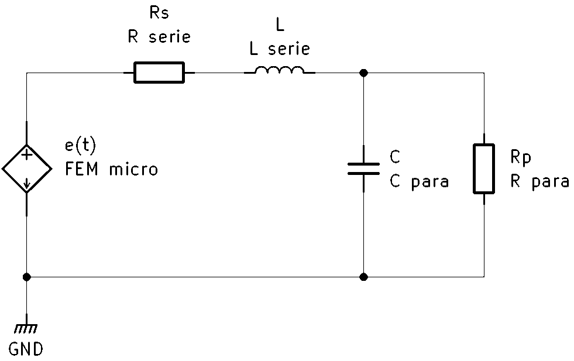
\includegraphics[width=0.8\textwidth]{../../../Attachment/Schema/01-Schema-eq-mic.png}
    \caption{Schéma électrique équivalent d'un micro non chargé}
\end{figure}

On peut alors calculer l'impédance du micro et on obtient :
\begin{equation}
|Z(j\omega)| = \frac{1}{\sqrt{\left(\frac{1}{R_p} + \frac{R_s}{R_s^2 + (L\omega)^2}\right)^2 + \left(C\omega - \frac{L\omega}{R_s^2 + (L\omega)^2}\right)^2}}
\end{equation}

En utilisation réelle, le micro est connecté à un amplificateur dont la résistance d'entrée est modélisée par une charge $R_{amp}$. L'étude de ce circuit permet d'établir la fonction de transfert $H(p) = \frac{u(p)}{e(p)}$. On obtient alors l'expression suivante :
\begin{equation}
H(p) = \frac{R_p R_{amp}}{R_p R_{amp} + R_s R_{amp} + R_s R_p} \frac{1}{1 + \frac{R_s R_p R_{amp} C + L R_{amp} + L R_p}{R_p R_{amp} + R_s R_{amp} + R_s R_p}p + \frac{R_p R_{amp} L C}{R_p R_{amp} + R_s R_{amp} + R_s R_p}p^2}
\end{equation}
Cette équation démontre que le micro, une fois chargé, se comporte comme un filtre passe-bas du second ordre.

\subsection{Expérimentation}
L'objectif de cette première phase expérimentale est de caractériser les paramètres physiques $R_s$, $L$, $C$, $R_p$ introduits dans le modèle théorique précédent (1.1). Ces valeurs, dépendantes de la géométrie et de la conception du bobinage, sont déterminées par une méthode d'identification fréquentielle.

\subsubsection{Protocole expérimental}
Le dispositif repose sur un montage en pont diviseur de tension. Le micro est placé en série avec une résistance de précision $R_{amp} = 100k\Omega$. En appliquant une tension sinusoïdale $U$ d'amplitude constante et de fréquence variable, nous mesurons la tension $V$ aux bornes du micro. Le module de l'impédance $|Z|$ du micro est alors extrait par la relation suivante : 
$$|Z| = \frac{V R_{amp}}{U-V}$$

\begin{figure}[H]
    \centering
    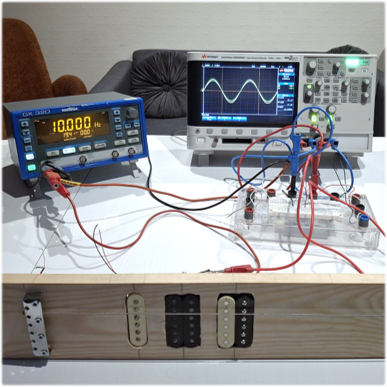
\includegraphics[width=0.8\textwidth]{../../../Test/Main/01-Elec.png}
    \caption{Photo du dispositif expérimental}
\end{figure}

\subsubsection{Traitement des données et optimisation}
La résistance série $R_s$ est mesurée préalablement en courant continu à l'aide d'un multimètre. Les autres paramètres $L$, $C$, $R_p$ sont obtenus par un ajustement numérique du modèle théorique sur les points expérimentaux (Fig. 3). Nous utilisons pour cela l'algorithme de moindre-carre, qui minimise l'écart quadratique entre la prédiction et la mesure (Fig. 4).

\subsubsection{Résultats}
Les résultats obtenus pour les deux types de micros étudiés sont regroupés dans le tableau ci-dessous :

\begin{center}
\begin{tabular}{lcccc}
\toprule
\textbf{Type de micro} & $\boldsymbol{R_s}$ & \textbf{L} & \textbf{C} & $\boldsymbol{R_p}$ \\
\midrule
SingleCoil & 5,26 k$\Omega$ & 2,37 H & 0,37 nF & 492,3 k$\Omega$ \\
Humbucker parallèle & 4,52 k$\Omega$ & 1,72 H & 0,05 nF & 343,0 k$\Omega$ \\
Humbucker série & 15,1 k$\Omega$ & 4,60 H & 0,11 nF & 1,05 M$\Omega$ \\
\bottomrule
\end{tabular}
\end{center}

L'examen des courbes d'impédance (Fig. 3) confirme la nature résonante des trois dispositifs étudiés : le SingleCoil, le Humbucker en configuration parallèle et le Humbucker en configuration série. Les résultats expérimentaux révèlent que la fréquence de résonance du Humbucker série est significativement plus élevée que celle du SingleCoil, en accord avec la faible valeur de sa capacité parasite (0,11 nF), identifiée par l'algorithme de moindre-carre. En revanche, le Humbucker parallèle, caractérisé par une capacité parasite de 0,05 nF et une inductance de 1,72 H, présente une résonance à une fréquence intermédiaire, distincte des deux autres configurations.

L'analyse détaillée des relevés expérimentaux met en évidence une asymétrie marquée dans la réponse fréquentielle du Humbucker parallèle, contrastant avec la symétrie du pic de résonance du SingleCoil et du Humbucker série.

\begin{figure}[H]
    \centering
    \begin{minipage}{0.48\textwidth}
        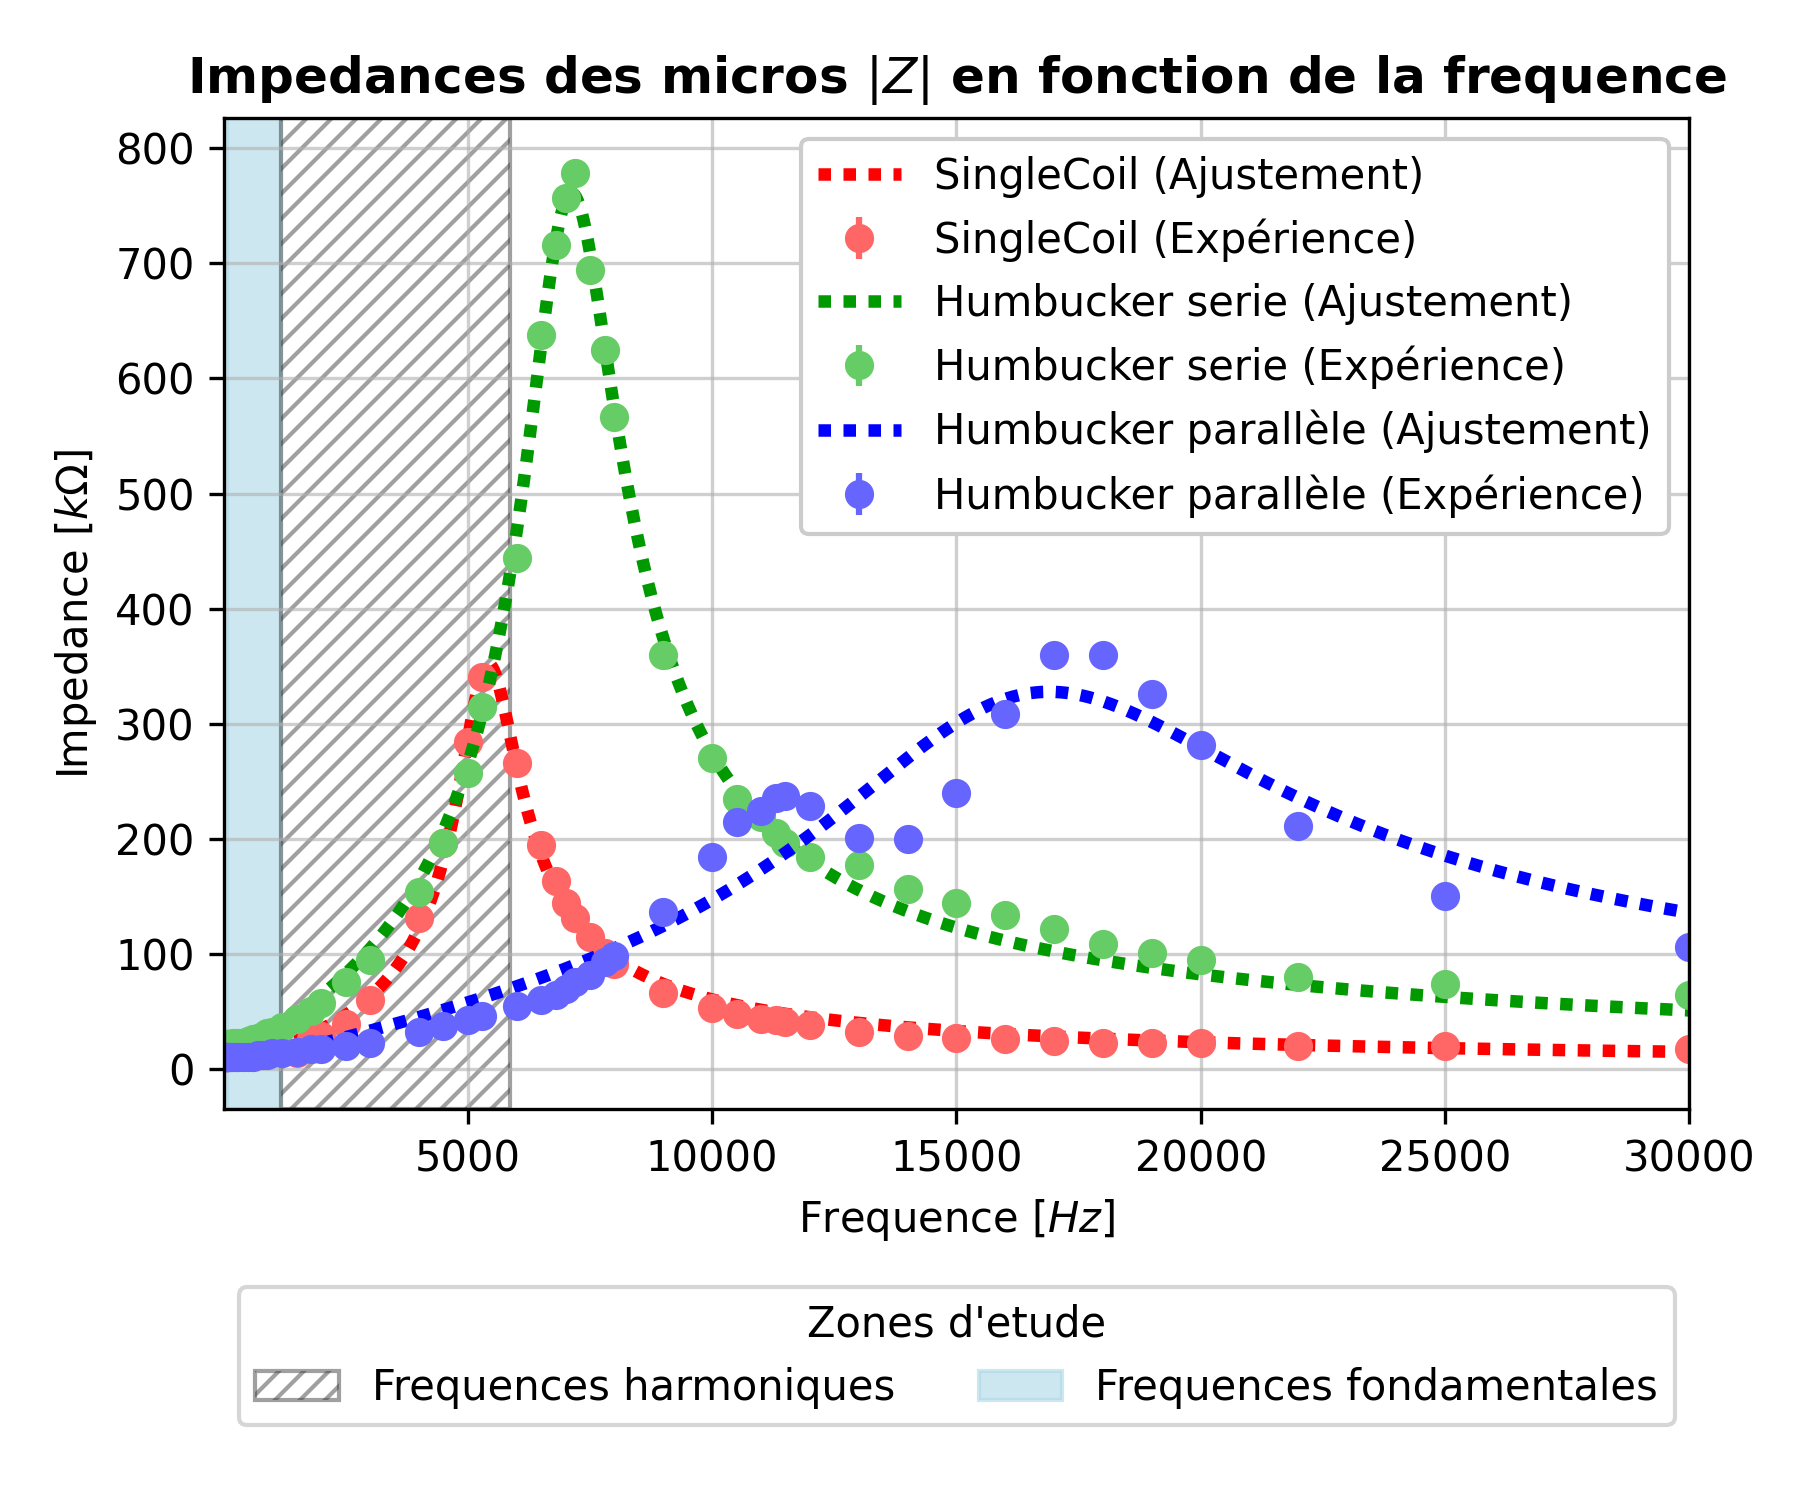
\includegraphics[width=\linewidth]{../../../Python/Exports/01-Reponse_electrique_frequetielle/Impedance.png}
        \caption{Relevé expérimentaux de l'impédance}
    \end{minipage}\hfill
    \begin{minipage}{0.48\textwidth}
        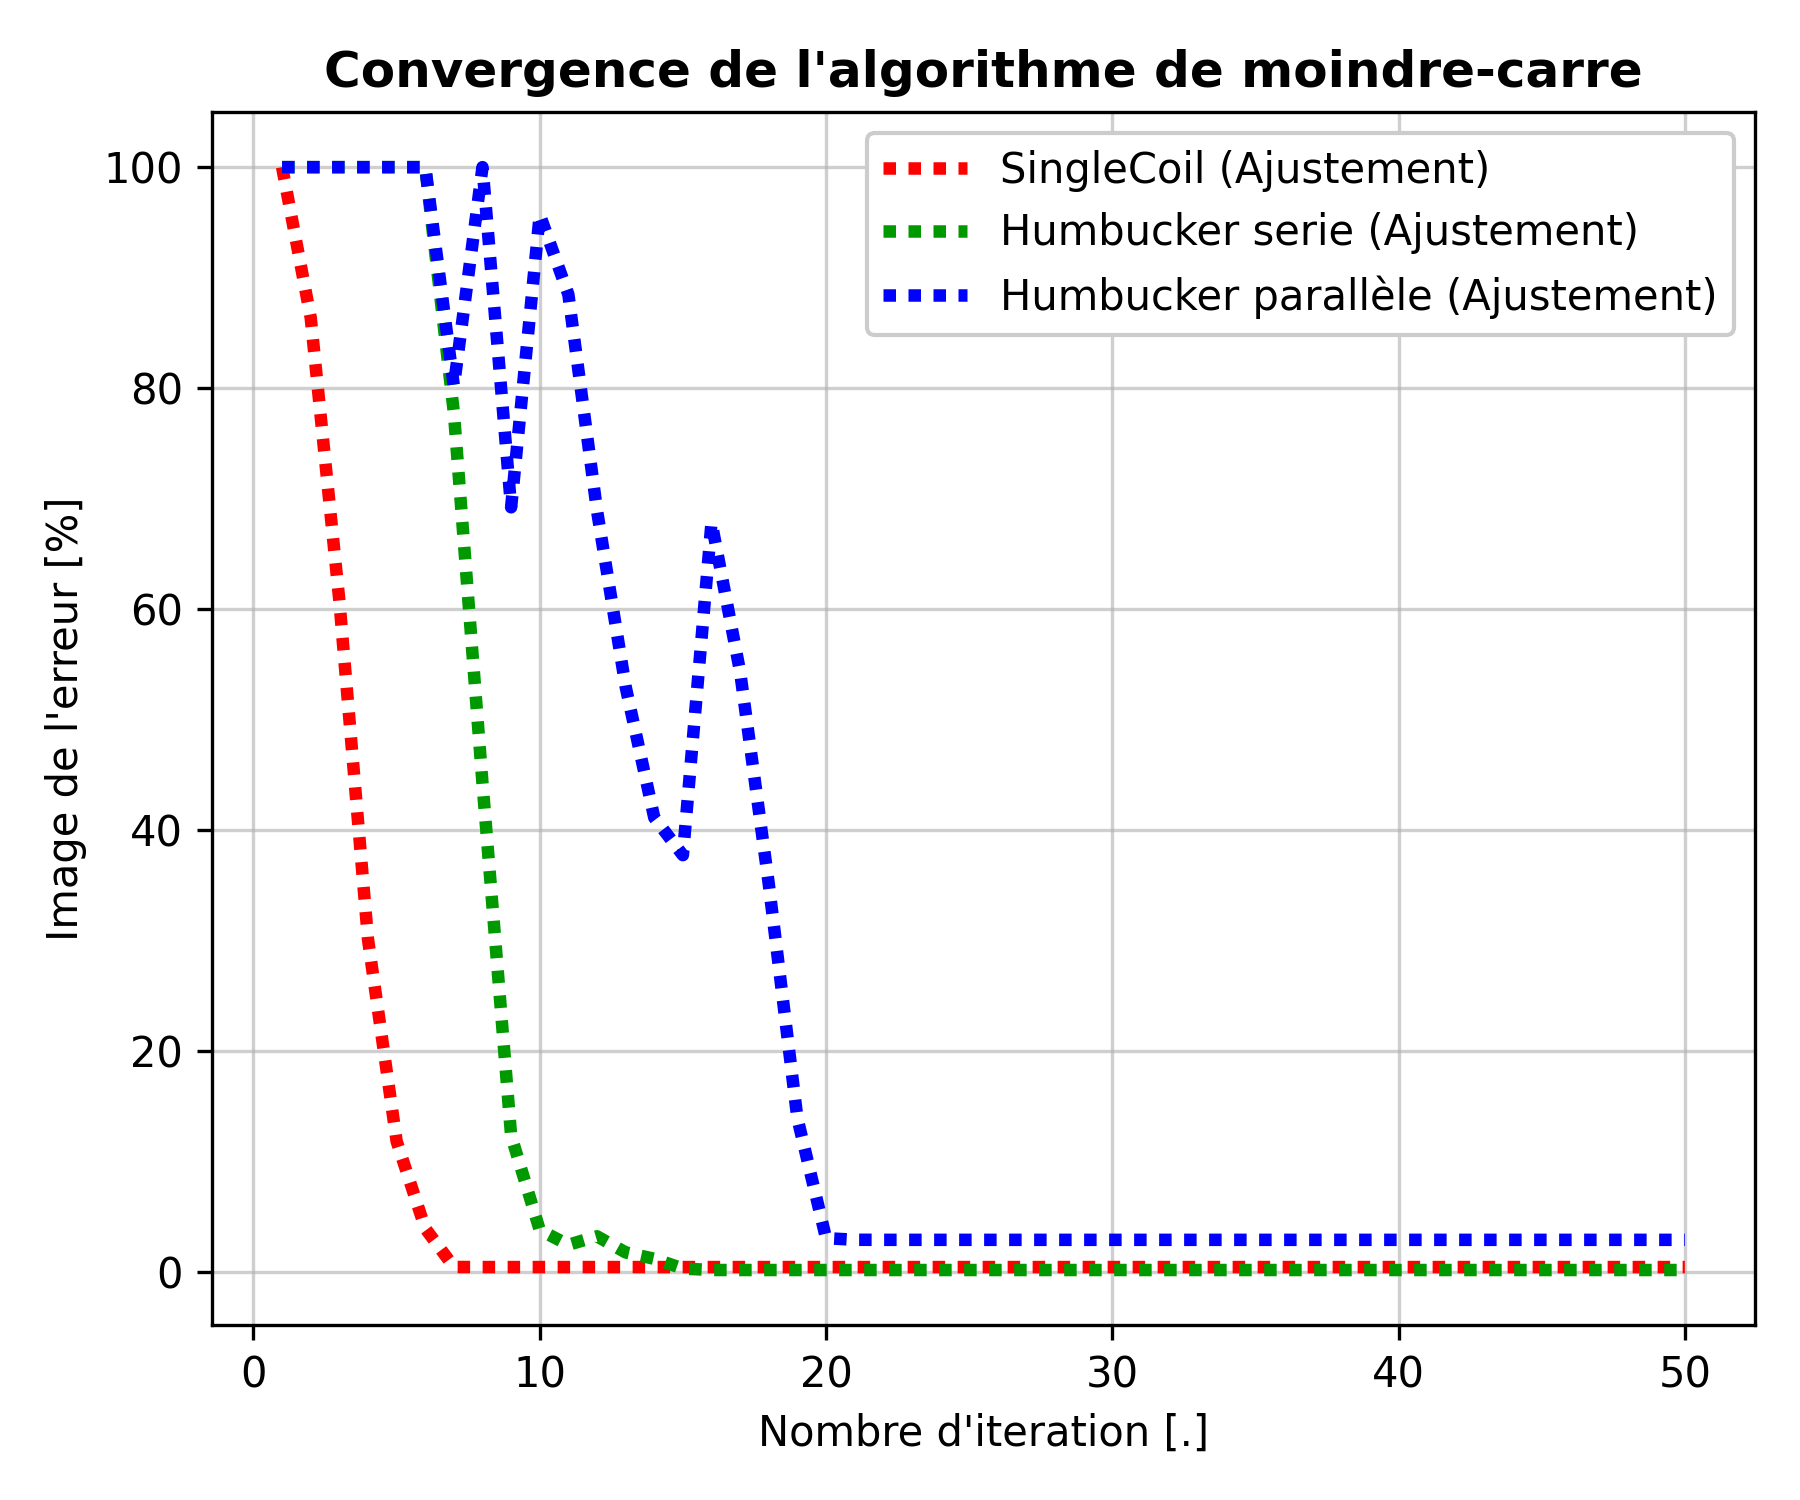
\includegraphics[width=\linewidth]{../../../Python/Exports/01-Reponse_electrique_frequetielle/Convergence.png}
        \caption{Convergence de l'algorithme de moindre-carre}
    \end{minipage}
\end{figure}

Cette singularité suggère que le modèle standard du second ordre, bien qu'adéquat pour décrire le SingleCoil et le Humbucker série, est insuffisant pour le Humbucker parallèle. L'allure de sa courbe d'impédance indique en effet un comportement compatible avec un système d'ordre 4, caractéristique d'un montage où les deux bobines ne sont pas identiques. Cette configuration modifie profondément la réponse fréquentielle du transducteur, en déplaçant la résonance vers les hautes fréquences et en introduisant une complexité supplémentaire dans le filtrage interne du signal.

L'identification des paramètres physiques permet désormais de simuler le comportement fréquentiel exact de chaque micro lorsqu'il est chargé par un amplificateur $R_{amp} = 1M\Omega$. La Figure 5 présente le diagramme de Bode obtenus par simulation numérique.

\begin{figure}[H]
    \centering
    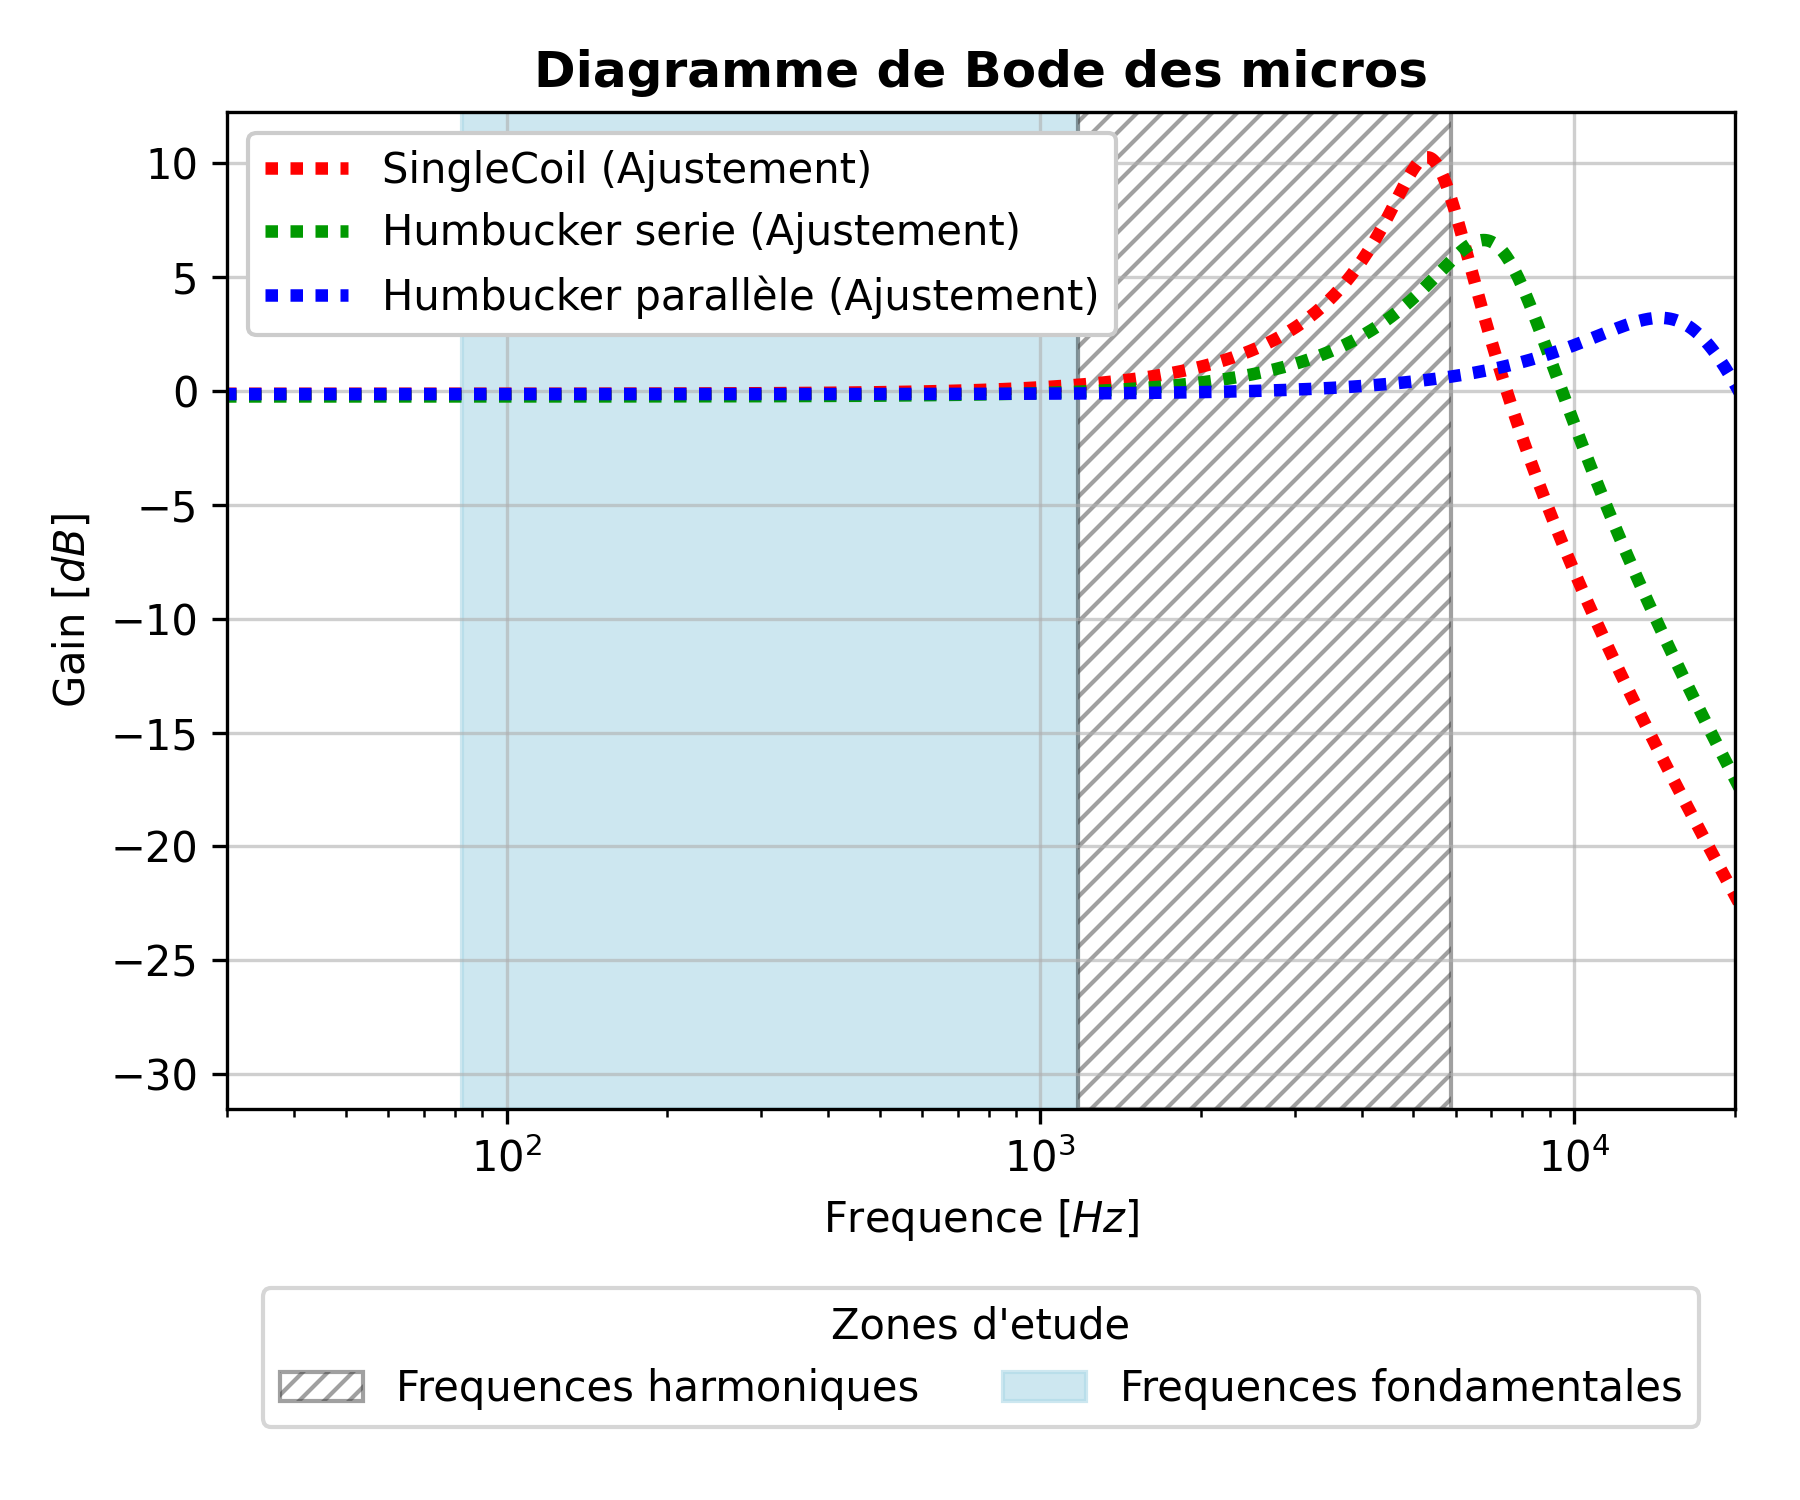
\includegraphics[width=0.8\textwidth]{../../../Python/Exports/01-Reponse_electrique_frequetielle/01-Gain.png}
    \caption{Diagramme de Bode des micros}
\end{figure}

\subsection{Conclusion}
Le micro SingleCoil se distingue par un pic de résonance marqué et un facteur de qualité élevé, favorisant une transmission sélective des harmoniques dans le haut du spectre audible. Cette caractéristique confère à ce type de bobinage sa sonorité << brillante >> et << tranchante >>, historiquement appréciée, où la surtension à la résonance enrichit le timbre original de la corde. 

À l'inverse, le Humbucker en configuration parallèle présente une réponse fréquentielle dépourvue de coloration harmonique dans les médiums et les aigus audibles. La résonance, rejetée vers des fréquences très élevées en raison de sa faible capacité parasite (0,05 nF), conduit à une restitution plus linéaire du signal, mais au détriment du renforcement des harmoniques aigües. Cette configuration engendre une perception sonore plus << sombre >> et moins riche en hautes fréquences, limitée par la bande passante du système d'amplification. 

Le Humbucker en configuration série, quant à lui, combine des éléments des deux comportements précédents. Avec une capacité parasite intermédiaire (0,11 nF) et une inductance plus élevée (4,60 H), il conserve une résonance plus marquée que le montage parallèle, tout en atténuant les harmoniques aigües par rapport au SingleCoil. Cette configuration offre ainsi un compromis entre la brillance du SingleCoil et la linéarité du Humbucker parallèle, avec une réponse fréquentielle plus équilibrée. 

Ces différences fondamentales entre les configurations de bobinage illustrent comment l'architecture électrique influence directement le timbre de la guitare. Le choix entre SingleCoil, Humbucker parallèle ou série dépendra donc des préférences sonores du musicien, ainsi que des contraintes techniques liées à l'environnement d'utilisation.

\newpage
% --- SECTION II ---
\section{Induction et filtrage spatial}

\subsection{Théorie}
\subsubsection{Vibration de la corde}
L'étude de la transduction électromagnétique repose sur la caractérisation précise de la vibration de la corde ferromagnétique et de son interaction avec le champ magnétique statique du micro. Conformément aux travaux de B. d'Andréa-Novel, B. Fabre et P. Jouvelot [6], le déplacement vertical de la corde $z(x,t)$ en un point $x$ et à un instant $t$ peut être modélisé par une superposition d'ondes stationnaires. L'expression générale du mouvement s'écrit alors :
\begin{equation}
z(x,t) = z_0 + \sum_{n} B_n \sin(k_n x) \cos(2\pi n F t)
\end{equation}
Dans cette équation, $z_0$ représente la position d'équilibre de la corde par rapport au micro, tandis que $B_n$ désigne l'amplitude de la $n^{\text{ième}}$ harmonique. Cette amplitude dépend étroitement des conditions initiales de pincement, notamment de l'amplitude initiale $A_0$ et de la position d'excitation $x_0$ le long de la longueur vibrante $L$. Le vecteur d'onde $k_n$ s'exprime ainsi : $k_n = n\pi/L$. La relation régissant ces amplitudes est la suivante :
\begin{equation}
B_n = \frac{A_0 L^{5/2} \sqrt{2}}{\pi^2 x_0 (L - x_0)} \frac{\sin\left(\frac{n\pi x_0}{L}\right)}{n^2}
\end{equation}

\subsubsection{Induction}
On considère une portion de la corde de volume $V$ et de susceptibilité magnétique $\chi$ placé dans le champ magnétique $\vec{B_m}$ de l'aimant permanent du micro. Ainsi, cette portion de corde acquiert un moment magnétique $\vec{m}$ tel que :
\begin{equation}
\vec{m} = \frac{\chi V \vec{B_m}}{\mu_0}
\end{equation}
Dans l'approximation dipolaire, et en considérant le moment magnétique aligné verticalement, le champ $\vec{B_c}$ créé par ce moment magnétique à une distance $z$ est donné par :
\begin{equation}
\vec{B_c}(z) = \frac{\mu_0}{4\pi} \frac{2\vec{m}}{z^3} = \frac{\chi V \vec{B_m}(z)}{2\pi z^3}
\end{equation}
Ainsi, le flux magnétique $\Phi$ traversant les $N$ spires de section $S$ s'exprime :
\begin{equation}
\Phi(z,t) = N \oint \vec{B_c}(z,t) \cdot \vec{dS} = \frac{N S \chi V}{2\pi} \frac{B_m(z)}{z(t)^3}
\end{equation}
L'application de la loi d'induction de Faraday permet finalement de déterminer la force électromotrice $e(x,t)$ induite dans le micro. En décomposant la dérivée temporelle du flux par la règle de la chaîne, soit $e(t) = -\frac{\partial\Phi}{\partial t} = -\frac{\partial\Phi}{\partial z}\frac{\partial z}{\partial t}$, nous obtenons l'expression finale du signal électrique :
\begin{equation}
e(x,t) = \frac{N S \chi V}{2\pi} \left( \frac{3B_m(z(t))}{z^4} - \frac{1}{z^3} \frac{\partial B_m}{\partial z}(t) \right) \sum_{n} B_n 2\pi n F \sin(k_n x) \sin(2\pi n F t)
\end{equation}
Ainsi, on a :
\begin{equation}
e(x,t) = \frac{N S \chi V}{2\pi} \left( \frac{3B_m(z(t))}{z^4} - \frac{1}{z^3} \frac{\partial B_m}{\partial z}(t) \right) \sum_{n} B_n A_n \sin(2\pi n F t)
\end{equation}
Cette formulation démontre que la tension induite est directement proportionnelle à la vitesse de vibration de la corde et dépend de la position spatiale du micro le long de celle-ci. Cette dépendance spatiale est à l'origine du phénomène de filtrage en peigne, qui sera analysé dans la section suivante pour comparer les micros SingleCoil et Humbucker.

\subsection{Expérimentation}
La validation du modèle d'induction repose sur une série de mesures temporelles et fréquentielles effectuées à l'aide d'une maquette de guitare instrumentée (Fig. 6). La corde, excitée manuellement, vibre à une fréquence fondamentale de 80 Hz. L'observation des signaux temporels (Fig. 7) met en évidence une corrélation globale entre la théorie et l'expérience, bien que des disparités morphologiques notables apparaissent, particulièrement à certaine fréquence spécifiques.

\begin{figure}[H]
    \centering
    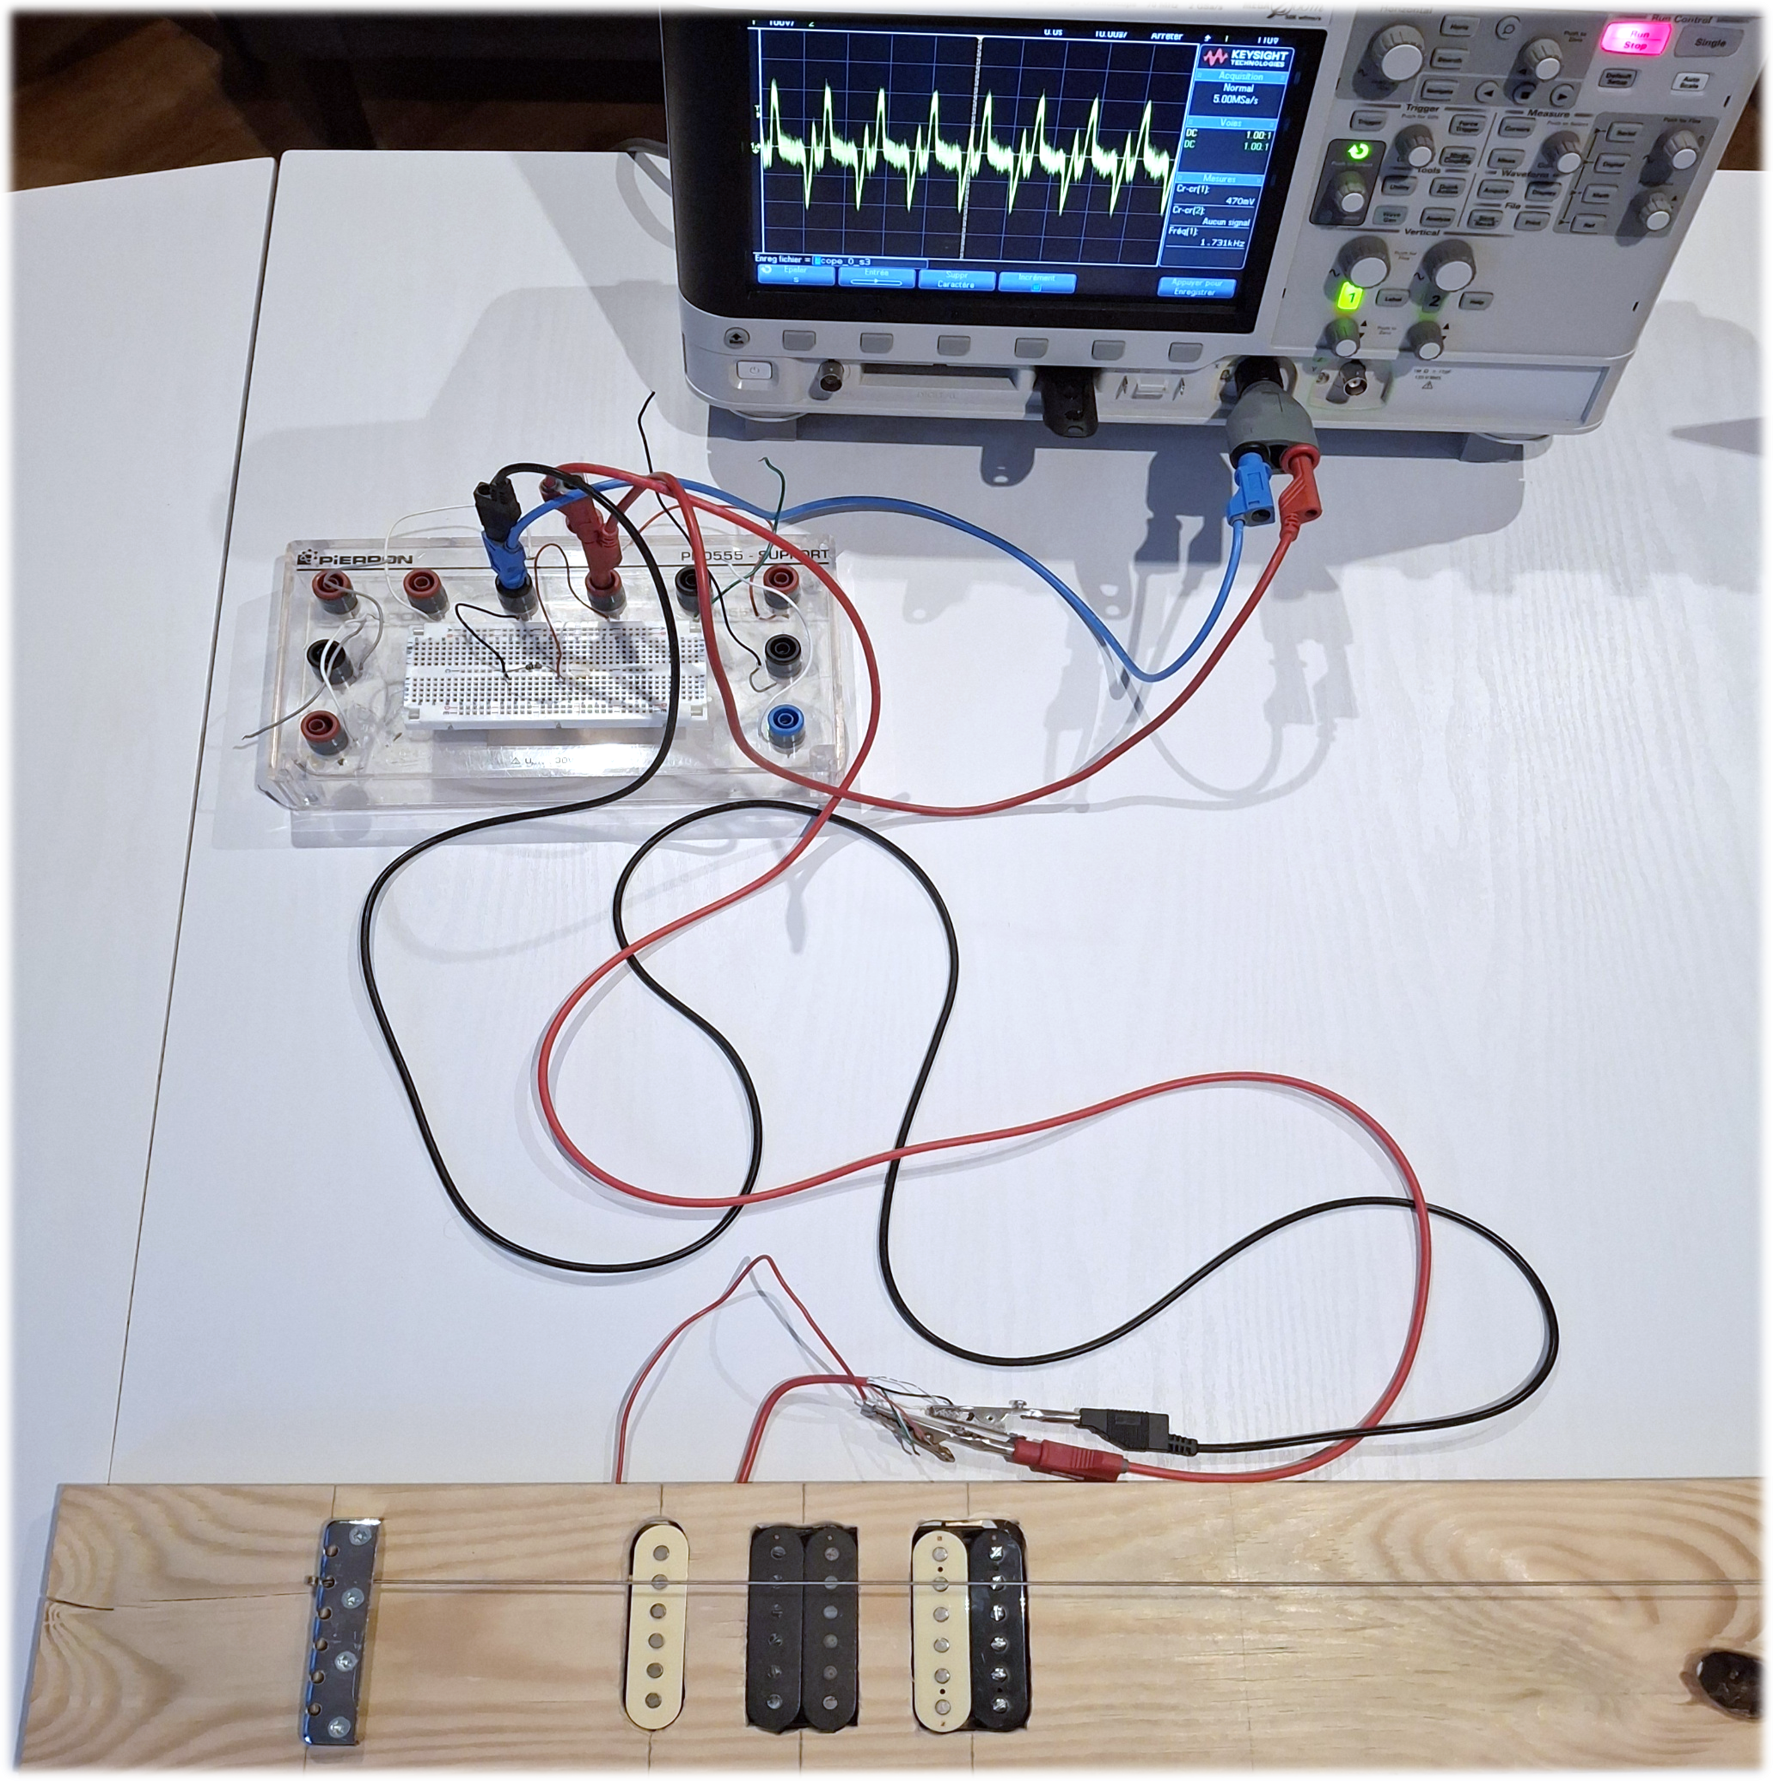
\includegraphics[width=0.5\textwidth]{../../../Test/Main/02-Meca.png}
    \caption{Photo du dispositif expérimental}
\end{figure}

\begin{figure}[H]
    \centering
    \begin{minipage}{0.48\textwidth}
        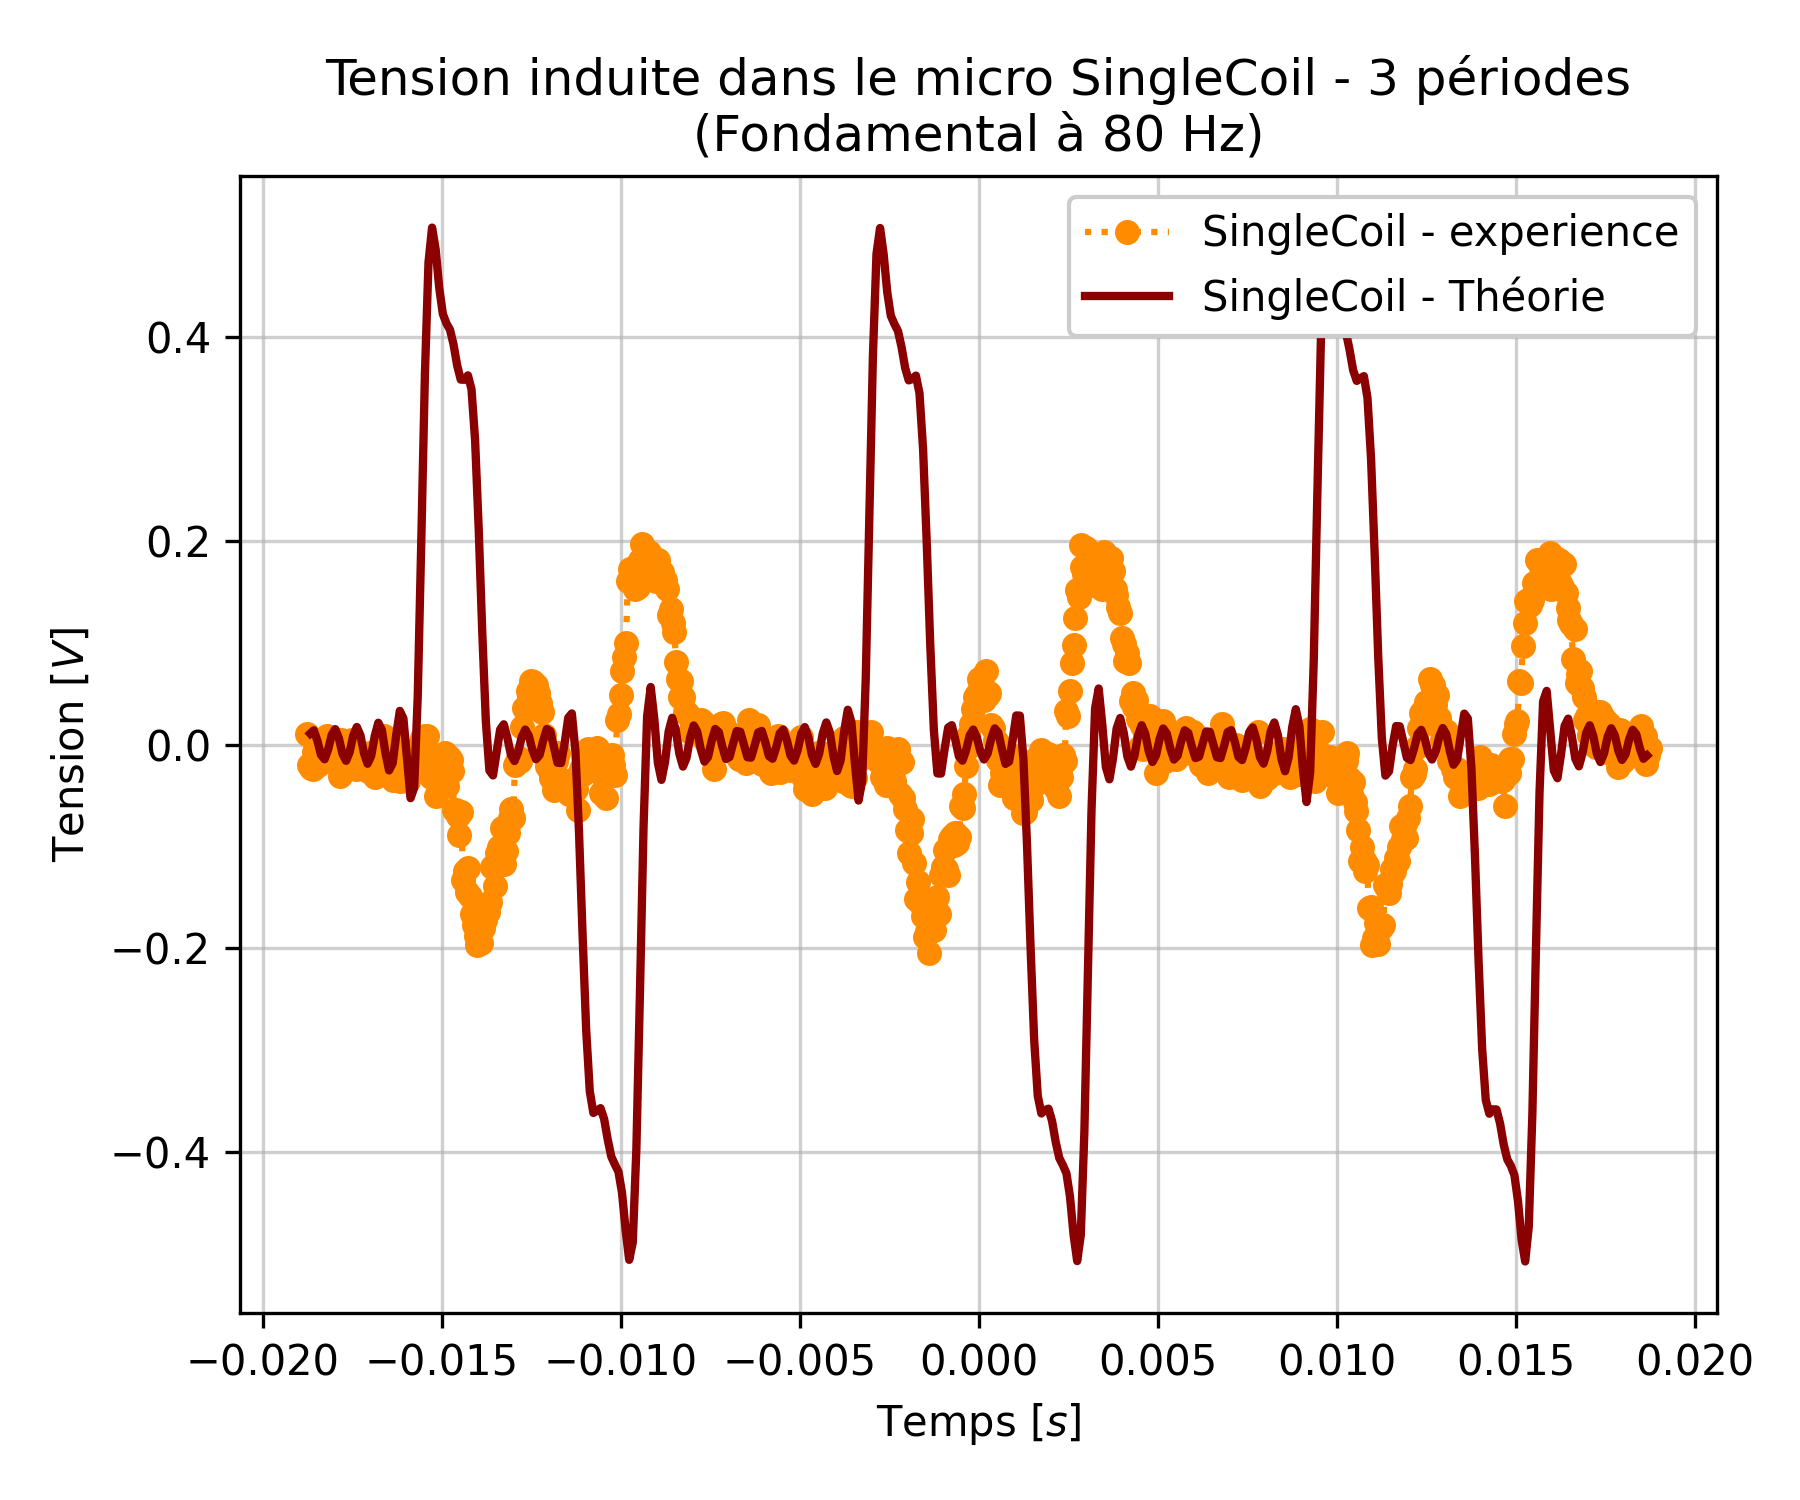
\includegraphics[width=\linewidth]{../../../Python/Exports/02-Reponse_mecanique/temporel/Singlecoil.png}
        \caption{Réponse temporelle du micro à une excitation de la corde}
    \end{minipage}\hfill
    \begin{minipage}{0.48\textwidth}
        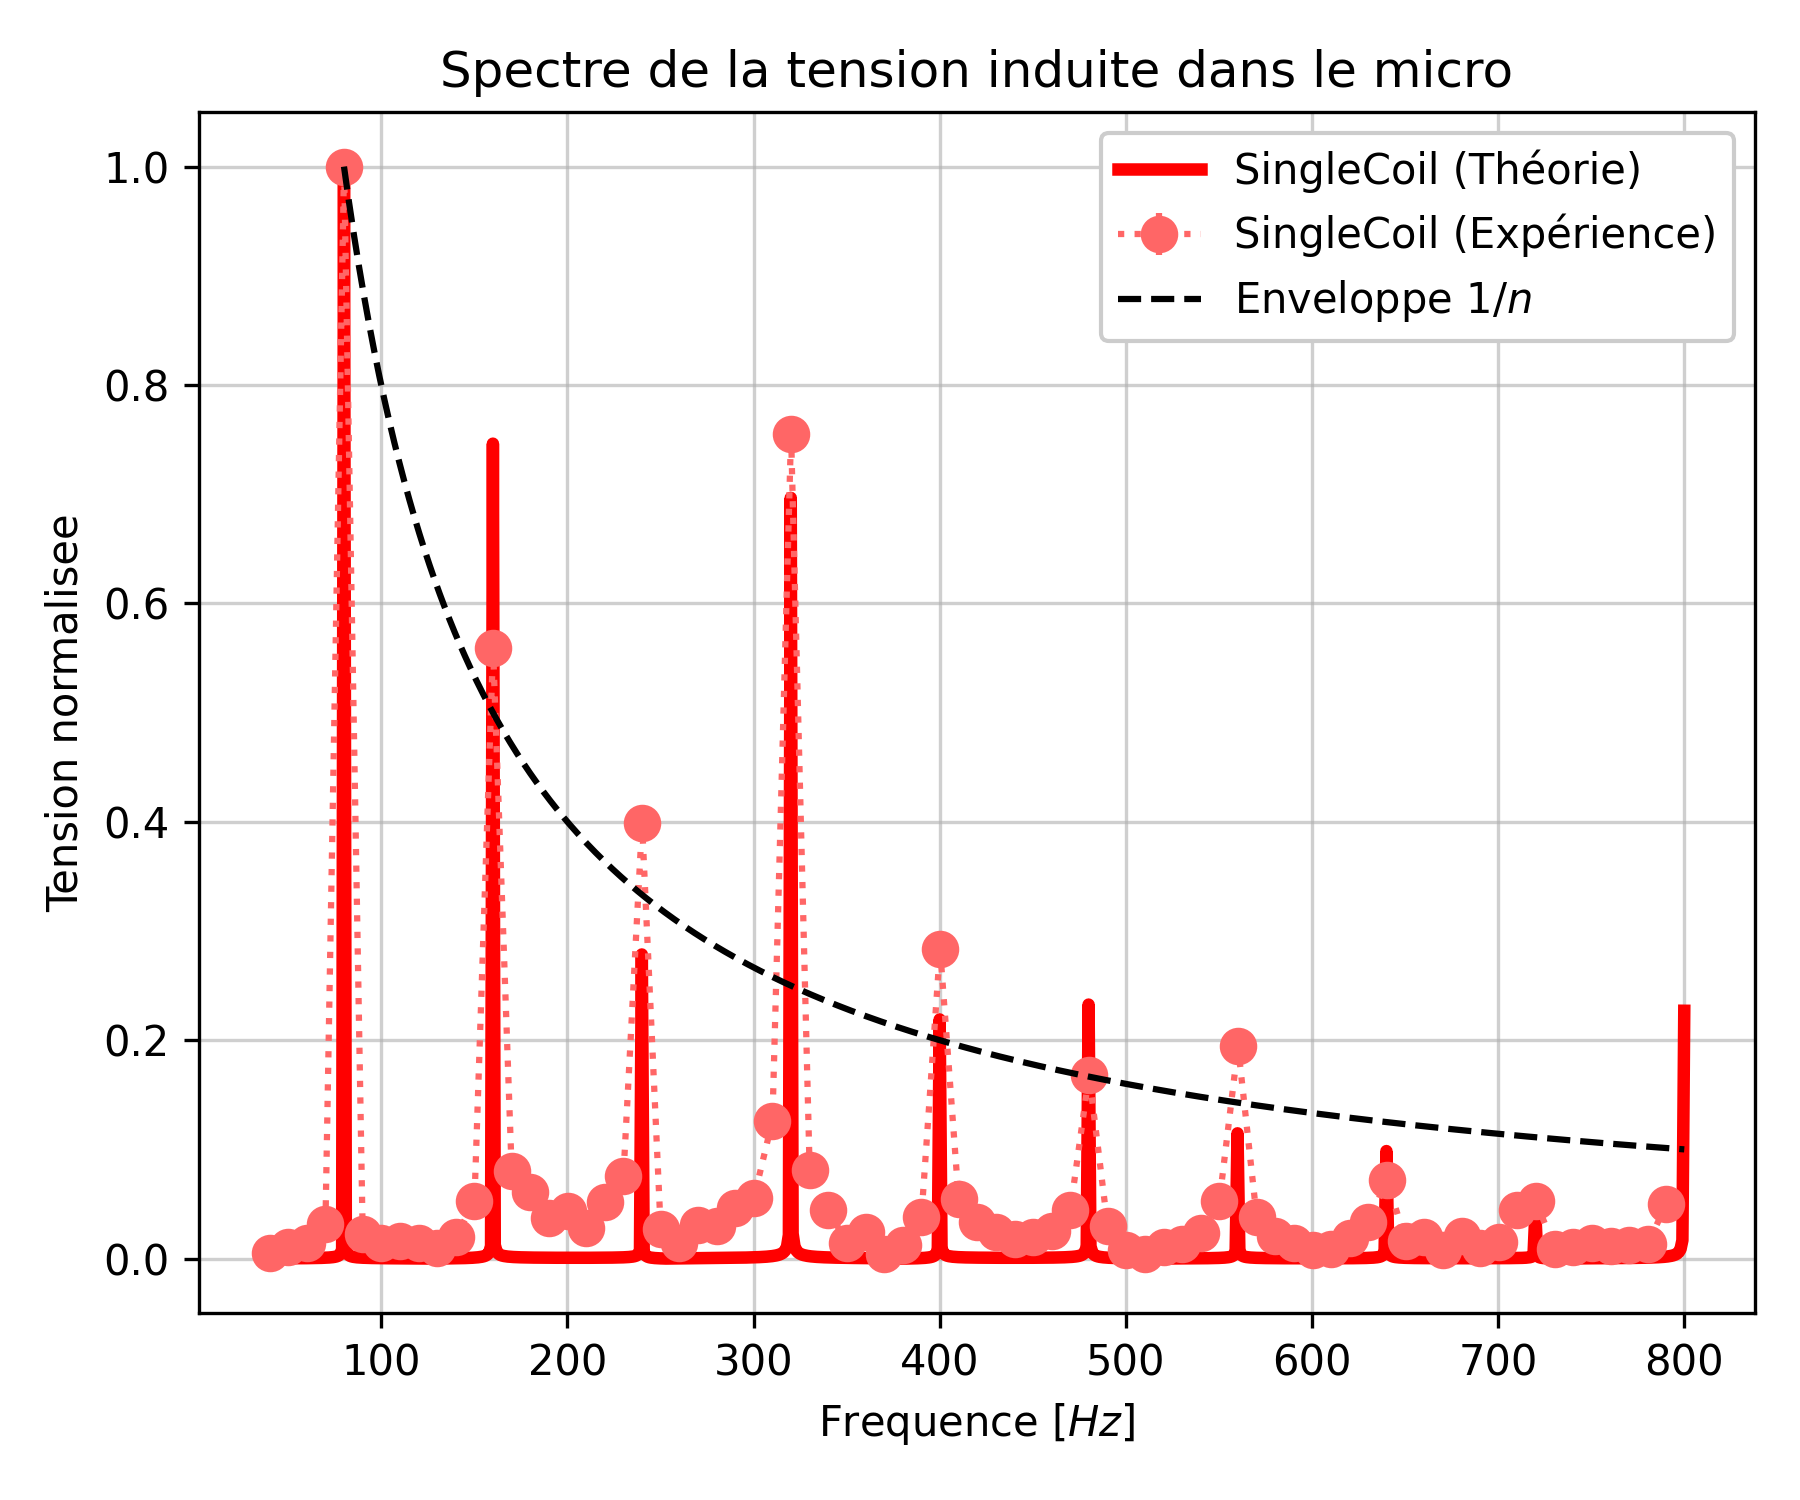
\includegraphics[width=\linewidth]{../../../Python/Exports/02-Reponse_mecanique/FFT/SC/Singlecoil.png}
        \caption{Réponse spectrale du micro à une excitation de la corde}
    \end{minipage}
\end{figure}

L'analyse spectrale des signaux (Fig. 8) confirme la présence des harmoniques de rang supérieur, conformément aux prédictions du développement en série de Fourier. Cependant, les amplitudes expérimentales divergent des valeurs théoriques issues du modèle dipolaire, en particulier pour certaines fréquences. Ces écarts s'expliquent par plusieurs phénomènes.

L'excitation manuelle de la corde introduit une condition initiale de pincement non idéalement triangulaire. Contrairement au modèle théorique, qui suppose une décroissance des amplitudes harmoniques en $1/n$, cette excitation génère un spectre harmonique plus riche et complexe, modifiant la répartition énergétique entre les fréquences fondamentales et leurs harmoniques. 

Le modèle théorique assimile le micro à un capteur ponctuel, négligeant ainsi l'intégration du flux magnétique sur la surface finie des plots. En réalité, la dimension non négligeable des bobines introduit un filtrage spatial passe-bas : les harmoniques dont la longueur d'onde est comparable à la taille du plot subissent une atténuation supplémentaire, altérant la réponse fréquentielle mesurée. 

Le modèle suppose un gradient de champ magnétique $\frac{\partial B_m}{\partial z}$ constant. Or, pour des amplitudes de vibration élevées, la corde pénètre dans des zones de saturation magnétique près des aimants, où le champ n'est plus linéaire. Ce phénomène induit une distorsion du signal temporel, se traduisant par des pics de tension plus << pointus >> et agressifs à l'oscilloscope, en contraste avec les courbes lissées des simulations.

\subsection{Conclusion}
L'étude comparative des technologies SingleCoil et Humbucker met en lumière l'impact déterminant de la géométrie du bobinage sur le timbre de la guitare électrique. Le SingleCoil, grâce à sa capture ponctuelle des vibrations, préserve l'intégralité du spectre harmonique, conférant au son sa brillance caractéristique et sa richesse en hautes fréquences. 

En revanche, le Humbucker, par sa structure double, introduit un filtrage en peigne spatial lié à l'espacement $\Delta$ entre ses deux bobines. Ce phénomène physique génère des interférences destructives pour les longueurs d'onde vibratoires dont les ventres se trouvent en opposition de phase entre les bobines. Ainsi, certaines harmoniques sont atténuées, agissant comme un égaliseur passif qui module activement le contenu spectral du signal.

\begin{figure}[H]
    \centering
    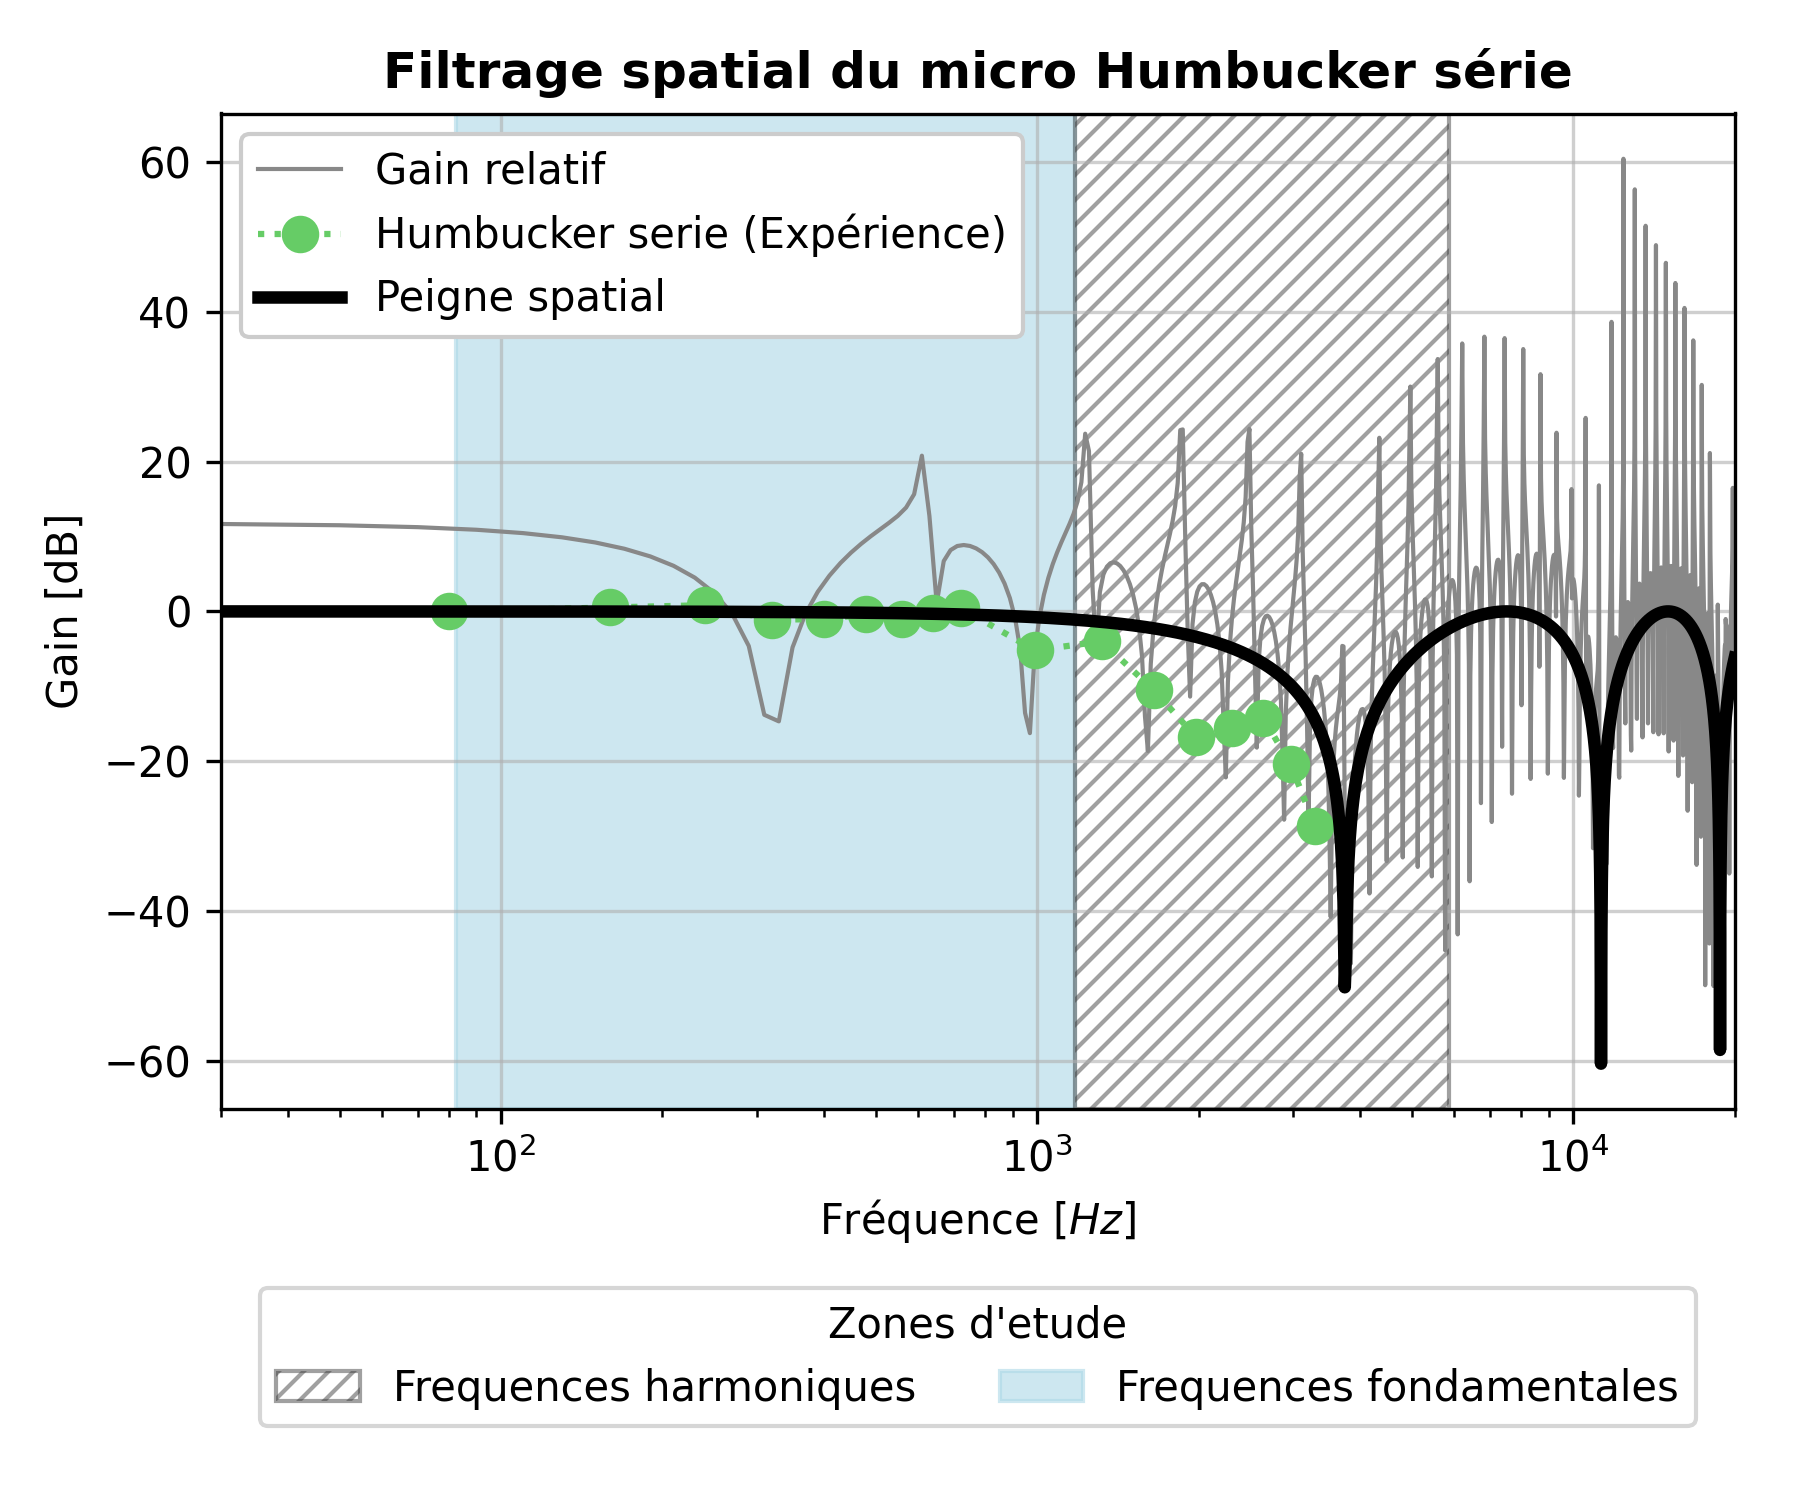
\includegraphics[width=0.8\textwidth]{../../../Python/Exports/02-Reponse_mecanique/Filtrage_spatial.png}
    \caption{Filtrage en peigne spatial du micro Humbucker}
\end{figure}

Ce filtrage spatial, combiné au filtrage électrique étudié en partie 1, explique scientifiquement la sonorité plus << mate >> et << ronde >> du Humbucker. La double bobine ne se limite donc pas à une simple réduction des parasites : elle redéfinit l'identité acoustique de l'instrument en altérant la structure même du signal induit, illustrant le compromis fondamental entre pureté sonore et richesse harmonique.

\newpage
% --- SECTION III ---
\section{Reduction du bourdonnement}

\subsection{Théorie}
L'étude de la sensibilité d'un capteur électromagnétique aux bruits environnants nécessite de modéliser le champ magnétique parasite comme un champ alternatif non uniforme. Dans le référentiel du micro, ce champ, induit principalement par le rayonnement du secteur à 50 Hz, est décrit par son amplitude locale $B_0$, sa fréquence $F_B$, et son gradient spatial $\alpha$ le long de l'axe longitudinal de la guitare. En ne considérant que la composante normale aux spires, l'expression simplifiée du champ parasite s'écrit :
\begin{equation}
B(x',t) = B_0(1 + \alpha x') \cos(2\pi F_B t)
\end{equation}
où $x'$ représente la position spatiale par rapport au centre de gravité du micro.

\subsubsection{Micro SingleCoil}
Dans la configuration d'un micro SingleCoil, le bobinage est centré en $x' = 0$. L'application de la loi d'induction de Lenz-Faraday permet d'exprimer la force électromotrice (f.e.m.) induite $e_S(t)$ en fonction du nombre de spires $N_S$ et de la surface active $S$. La f.e.m. résultante est alors directement proportionnelle à l'amplitude du champ incident :
\begin{equation}
e_S(t) = N_S S B_0 2\pi F_B \sin(2\pi F_B t)
\end{equation}
Ce résultat démontre l'absence de filtrage intrinsèque, le micro captant l'intégralité du bruit électromagnétique ambiant, ce qui génère le bourdonnement caractéristique observé expérimentalement (Fig. 11).

\subsubsection{Micro Humbucker}
Le micro Humbucker repose sur un principe de câblage en opposition de phase de deux bobines identiques, espacées d'une distance $\Delta$. La f.e.m. totale $e_H(t)$ est alors la différence des tensions induites dans chaque bobine, placées respectivement en $x'_1 = \frac{\Delta}{2}$ et $x'_2 = -\frac{\Delta}{2}$. Par sommation algébrique des contributions, les termes constants en $B_0$ s'annulent mutuellement par opposition de phase. Seul subsiste un terme résiduel dépendant du gradient spatial du champ :
\begin{equation}
e_{HS}(t) = N_{HS} S B_0 2\pi F_B \alpha \Delta \sin(2\pi F_B t)
\end{equation}
\begin{equation}
e_{HP}(t) = \frac{1}{2} N_{HP} S B_0 2\pi F_B \alpha \Delta \sin(2\pi F_B t)
\end{equation}
Cette démonstration met en évidence l'efficacité du Humbucker : dans un champ parfaitement uniforme ($\alpha = 0$), le bruit parasite est théoriquement nul. En pratique, le champ parasite présente toujours une légère inhomogénéité, mais le terme demeure très inférieur à l'unité, assurant ainsi une atténuation massive du bruit par rapport au micro SingleCoil. Cette propriété de rejection de mode commun constitue l'avantage technique majeur de ce type de bobinage dans les environnements électromagnétiques pollués.

\subsection{Expérimentation}
\subsubsection{Montage et protocole}
Afin de valider le modèle théorique de la rejection de mode commun, un dispositif expérimental s'appuyant sur un système de bobines de Helmholtz a été mis en œuvre (figure 10). Ce montage permet de générer, au centre du dispositif, un champ magnétique alternatif dont l'amplitude et la fréquence sont contrôlées avec précision par un générateur de fonctions (GBF). En plaçant les micros au centre de ces bobines, on assure un environnement où le champ magnétique est quasi uniforme, ce qui tend à minimiser le gradient spatial $\alpha$ conformément aux hypothèses théoriques précédemment établies. Pour simuler des conditions d'utilisation réelles, les micros sont connectés à une résistance de charge $R_{amp}$ de 1 M$\Omega$, modélisant l'impédance d'entrée d'un amplificateur standard, et la tension induite $u(t)$ est relevée aux bornes de cette résistance à l'aide d'un oscilloscope.

\begin{figure}[H]
    \centering
    \includegraphics[width=0.8\textwidth]{PATH}
    \caption{Photo du dispositif expérimental}
\end{figure}

\subsubsection{Résultats temporel}
La sensibilité des micros aux champs extérieurs est caractérisée par un coefficient de proportionnalité $k$ tel que :
\begin{equation}
|e| = k |B|
\end{equation}
Les mesures effectuées sous un champ parasite d'amplitude variable à une fréquence de 50 Hz révèlent une disparité majeure entre les deux technologies (Fig. 11).

\begin{figure}[H]
    \centering
    \begin{minipage}{0.48\textwidth}
        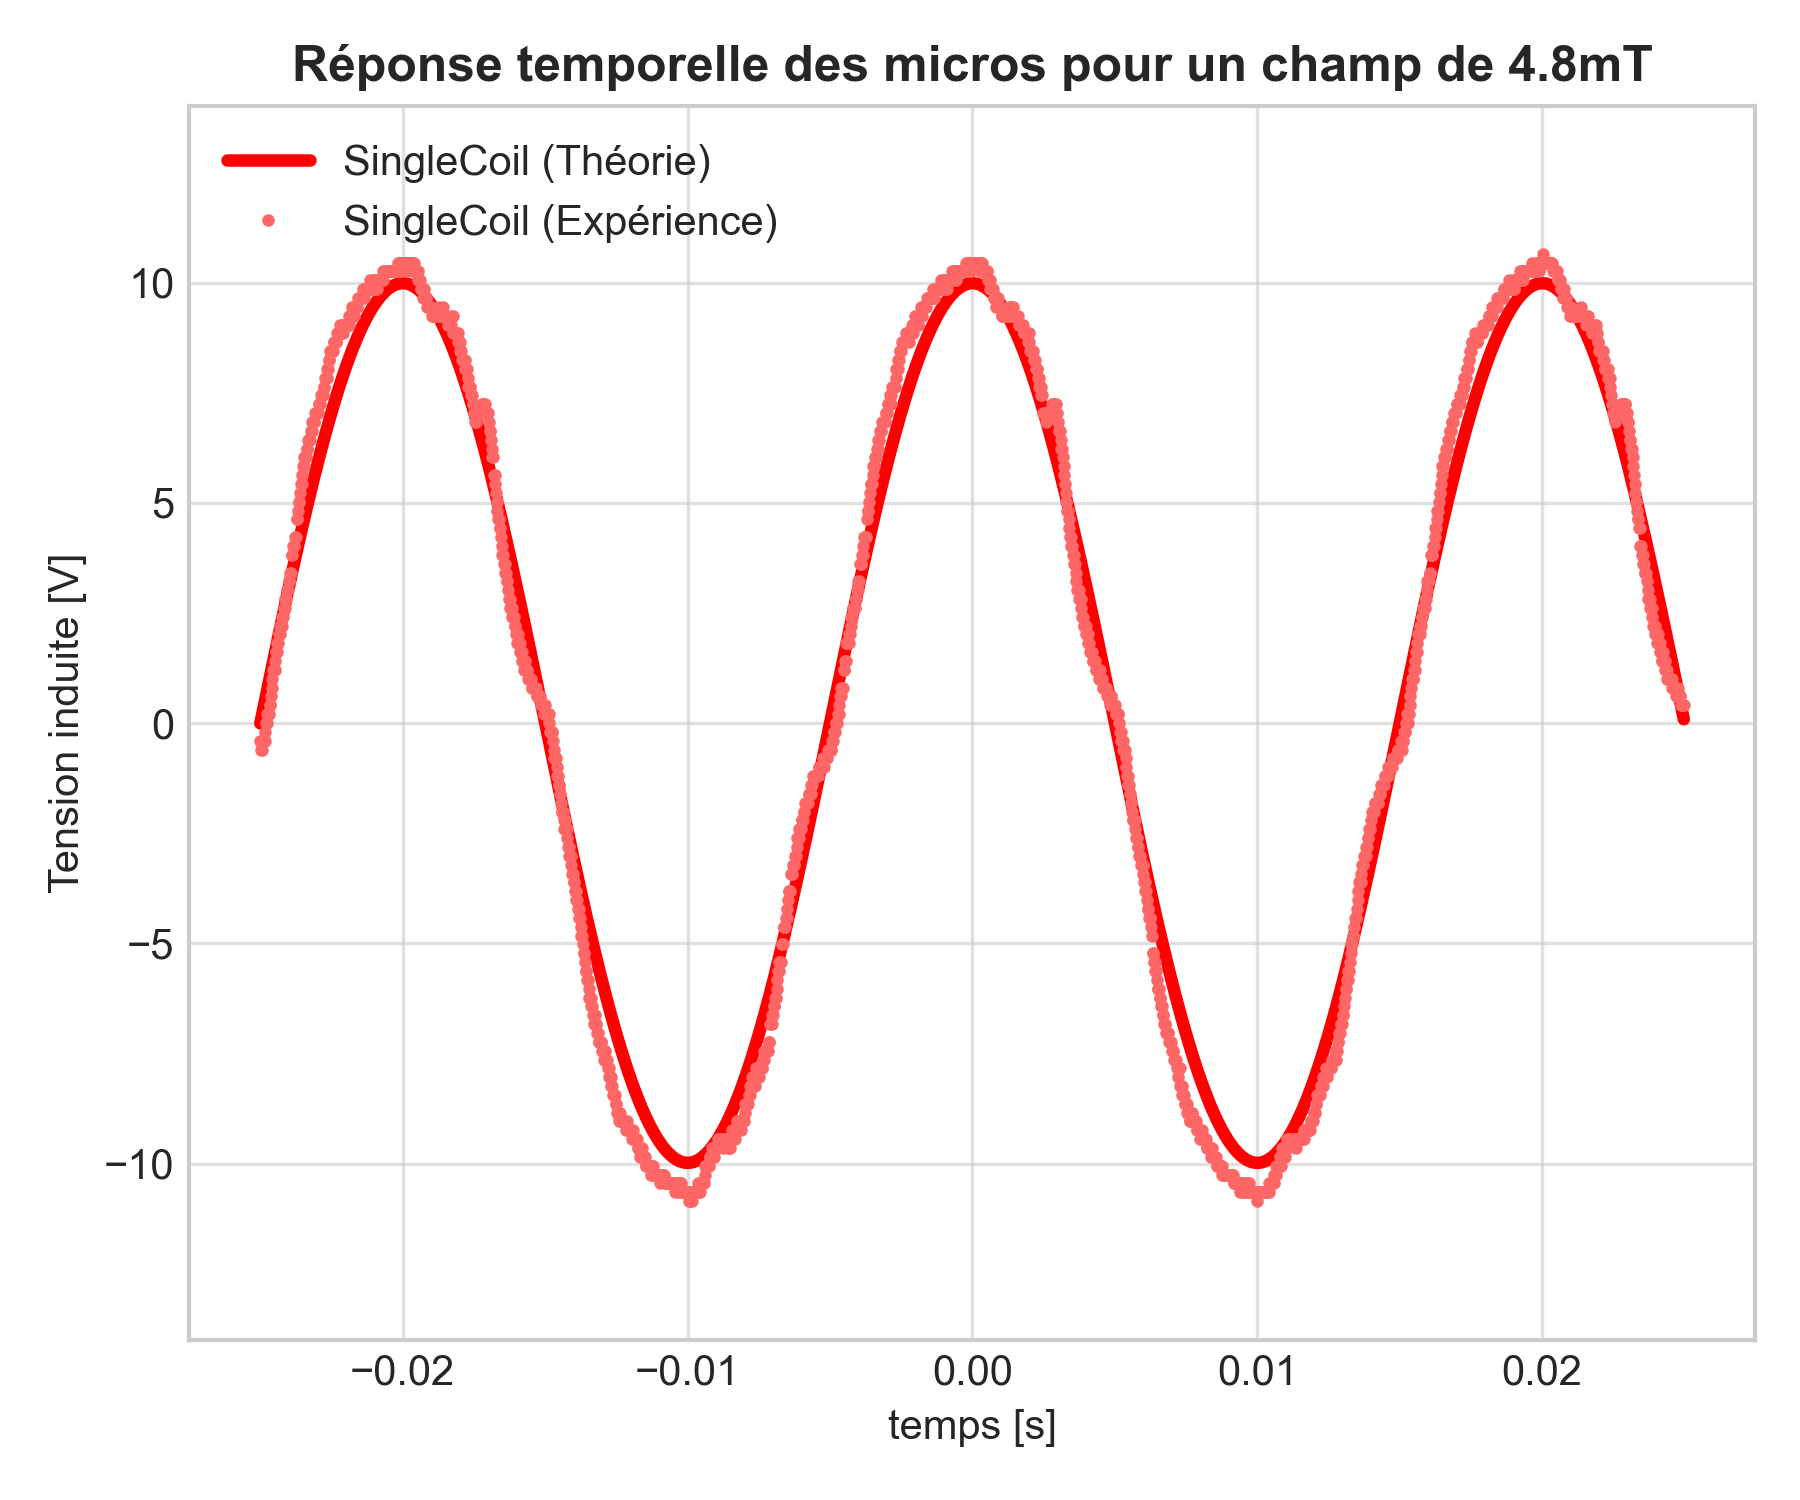
\includegraphics[width=\linewidth]{../../../Python/Exports/03-Reponse_magnetique/Singlecoil.png}
        \caption{Réponse temporelle du micro à un champ magnétique extérieur}
    \end{minipage}\hfill
    \begin{minipage}{0.48\textwidth}
        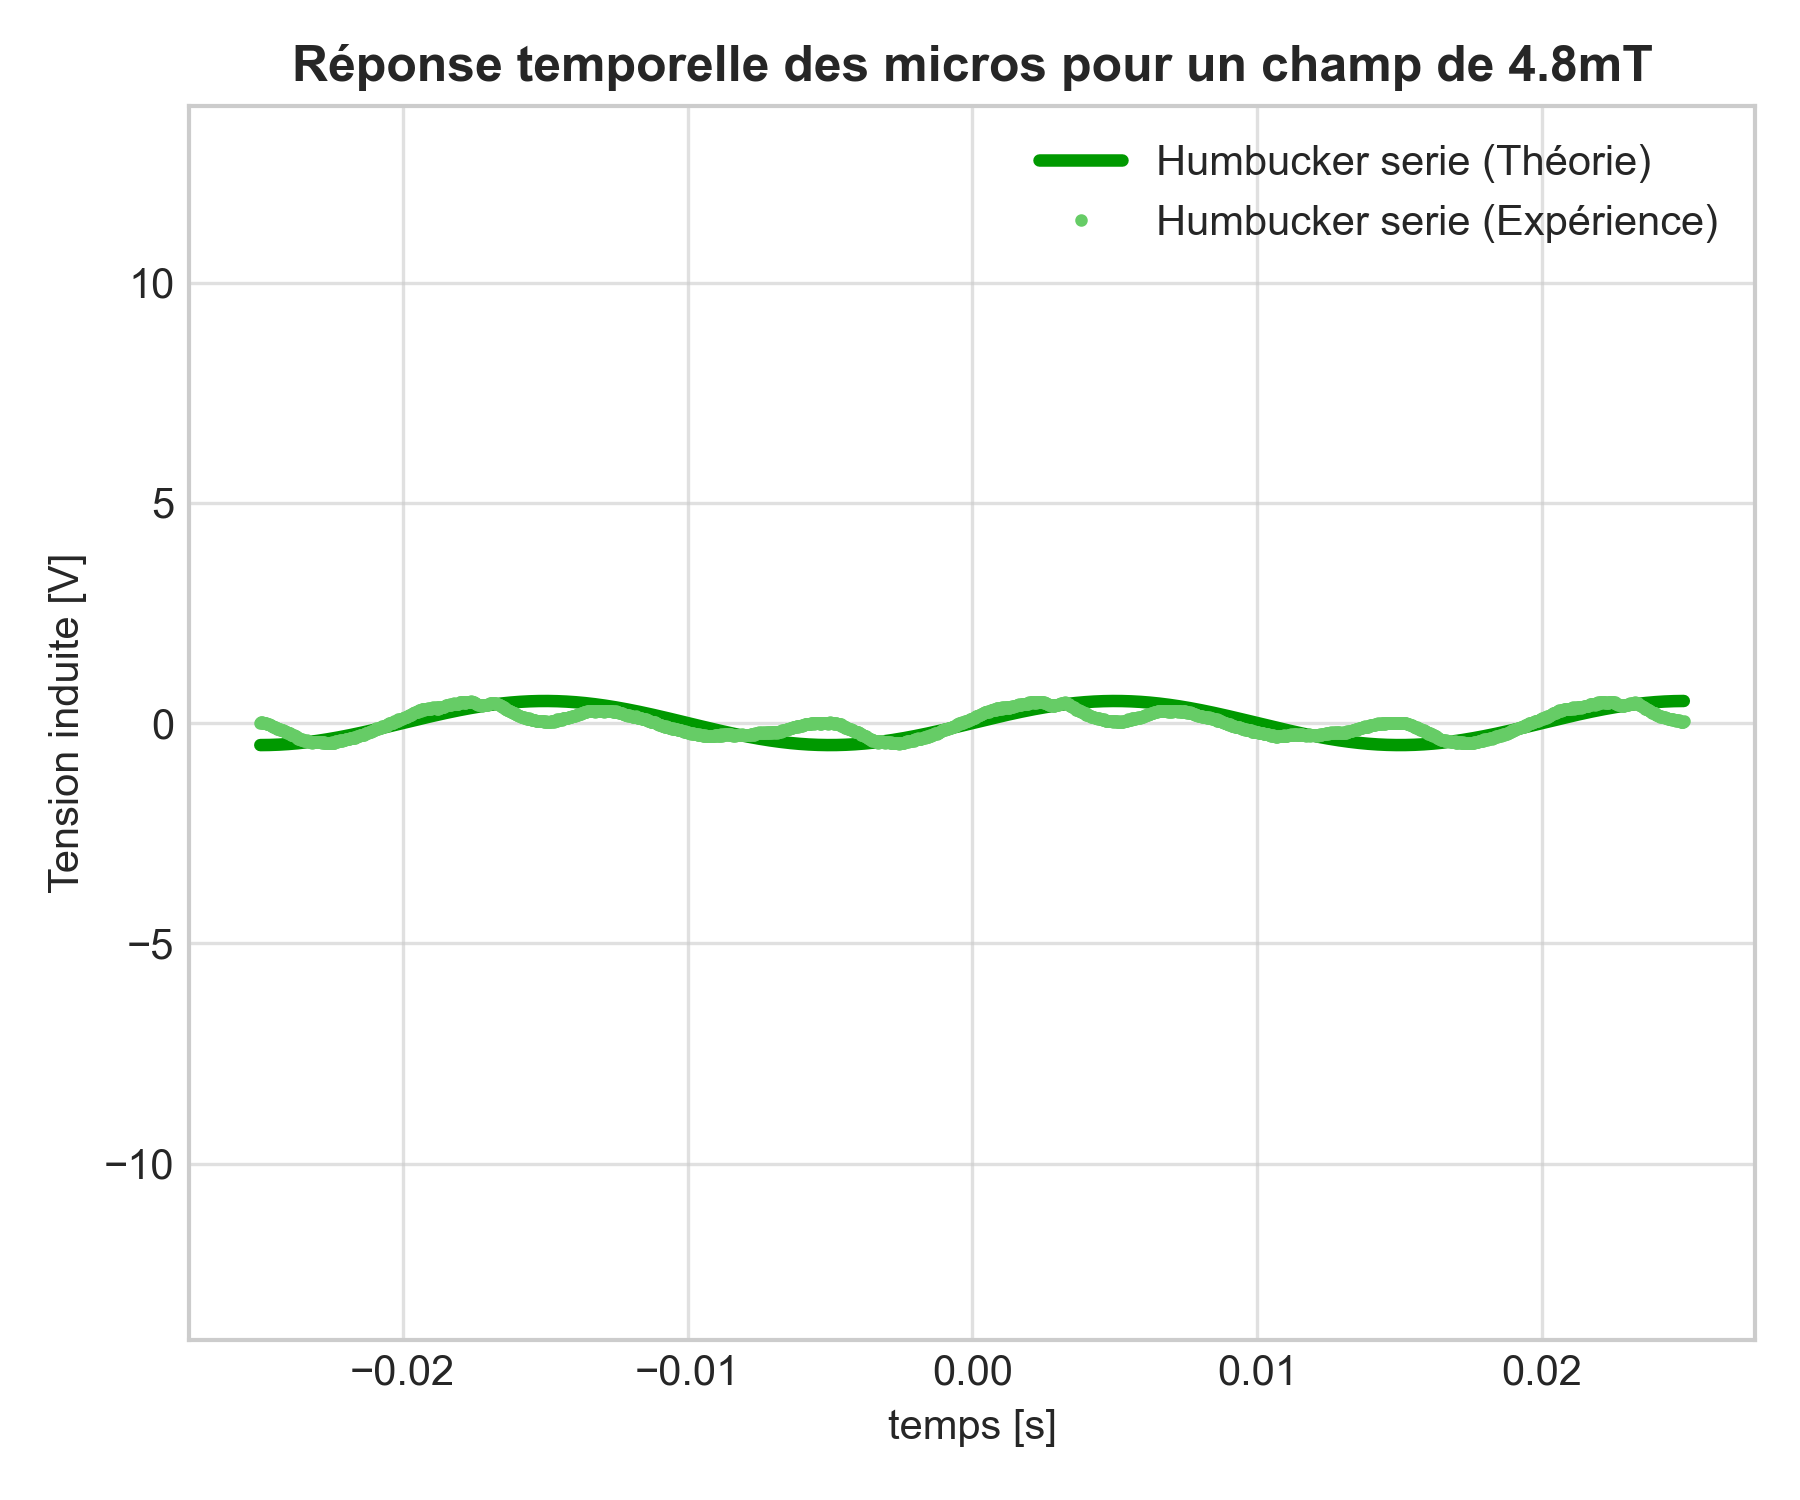
\includegraphics[width=\linewidth]{../../../Python/Exports/03-Reponse_magnetique/Humbucker.png}
        \caption{Réponse temporelle du micro à un champ magnétique extérieur}
    \end{minipage}
\end{figure}

\subsubsection{Taux de rejection de mode commun (CMRR)}
Les mesures expérimentales révèlent une sensibilité aux champs magnétiques parasites de $k_{Sexp} = 2,05 \text{ V}\cdot\text{mT}^{-1}$ pour le SingleCoil, contre $k_{Hpexp} = 1,37 \text{ V}\cdot\text{mT}^{-1}$ pour le Humbucker parallèle et $k_{Hsexp} = 0,08 \text{ V}\cdot\text{mT}^{-1}$  (Fig. 12). Bien que cette atténuation confirme l'efficacité relative du Humbucker, la valeur absolue de $k_{Hpexp}$ reste élevée, ce qui corrobore l'idée selon laquelle le micro testé adopte une asymétrie de bobinage.

Ce réduction de sensibilité est quantifiée par le taux de rejection de mode commun (CMRR). L'écart significatif entre le CMRR théorique (39,3 dB) et la valeur expérimentale (3,5 dB) met en évidence les limites pratiques de l'annulation parfaite des parasites. Plusieurs facteurs expliquent cette divergence comme l'asymétries de construction des bobinages détecté en partie I ou encore l'imperfections du montage expérimental, introduisant des dissymétries dans l'exposition au champ parasite.

Malgré ces limitations, les résultats valident la supériorité du Humbucker pour la préservation de la pureté du signal en environnement bruité, notamment face aux interférences magnétiques de basse fréquence (ex: 50 Hz). Cette étude souligne ainsi l'importance du design mécanique et électrique dans l'optimisation des performances antiparasites, tout en confirmant que les modèles théoriques idéaux doivent être adaptés aux contraintes réelles de fabrication.

\begin{figure}[H]
    \centering
    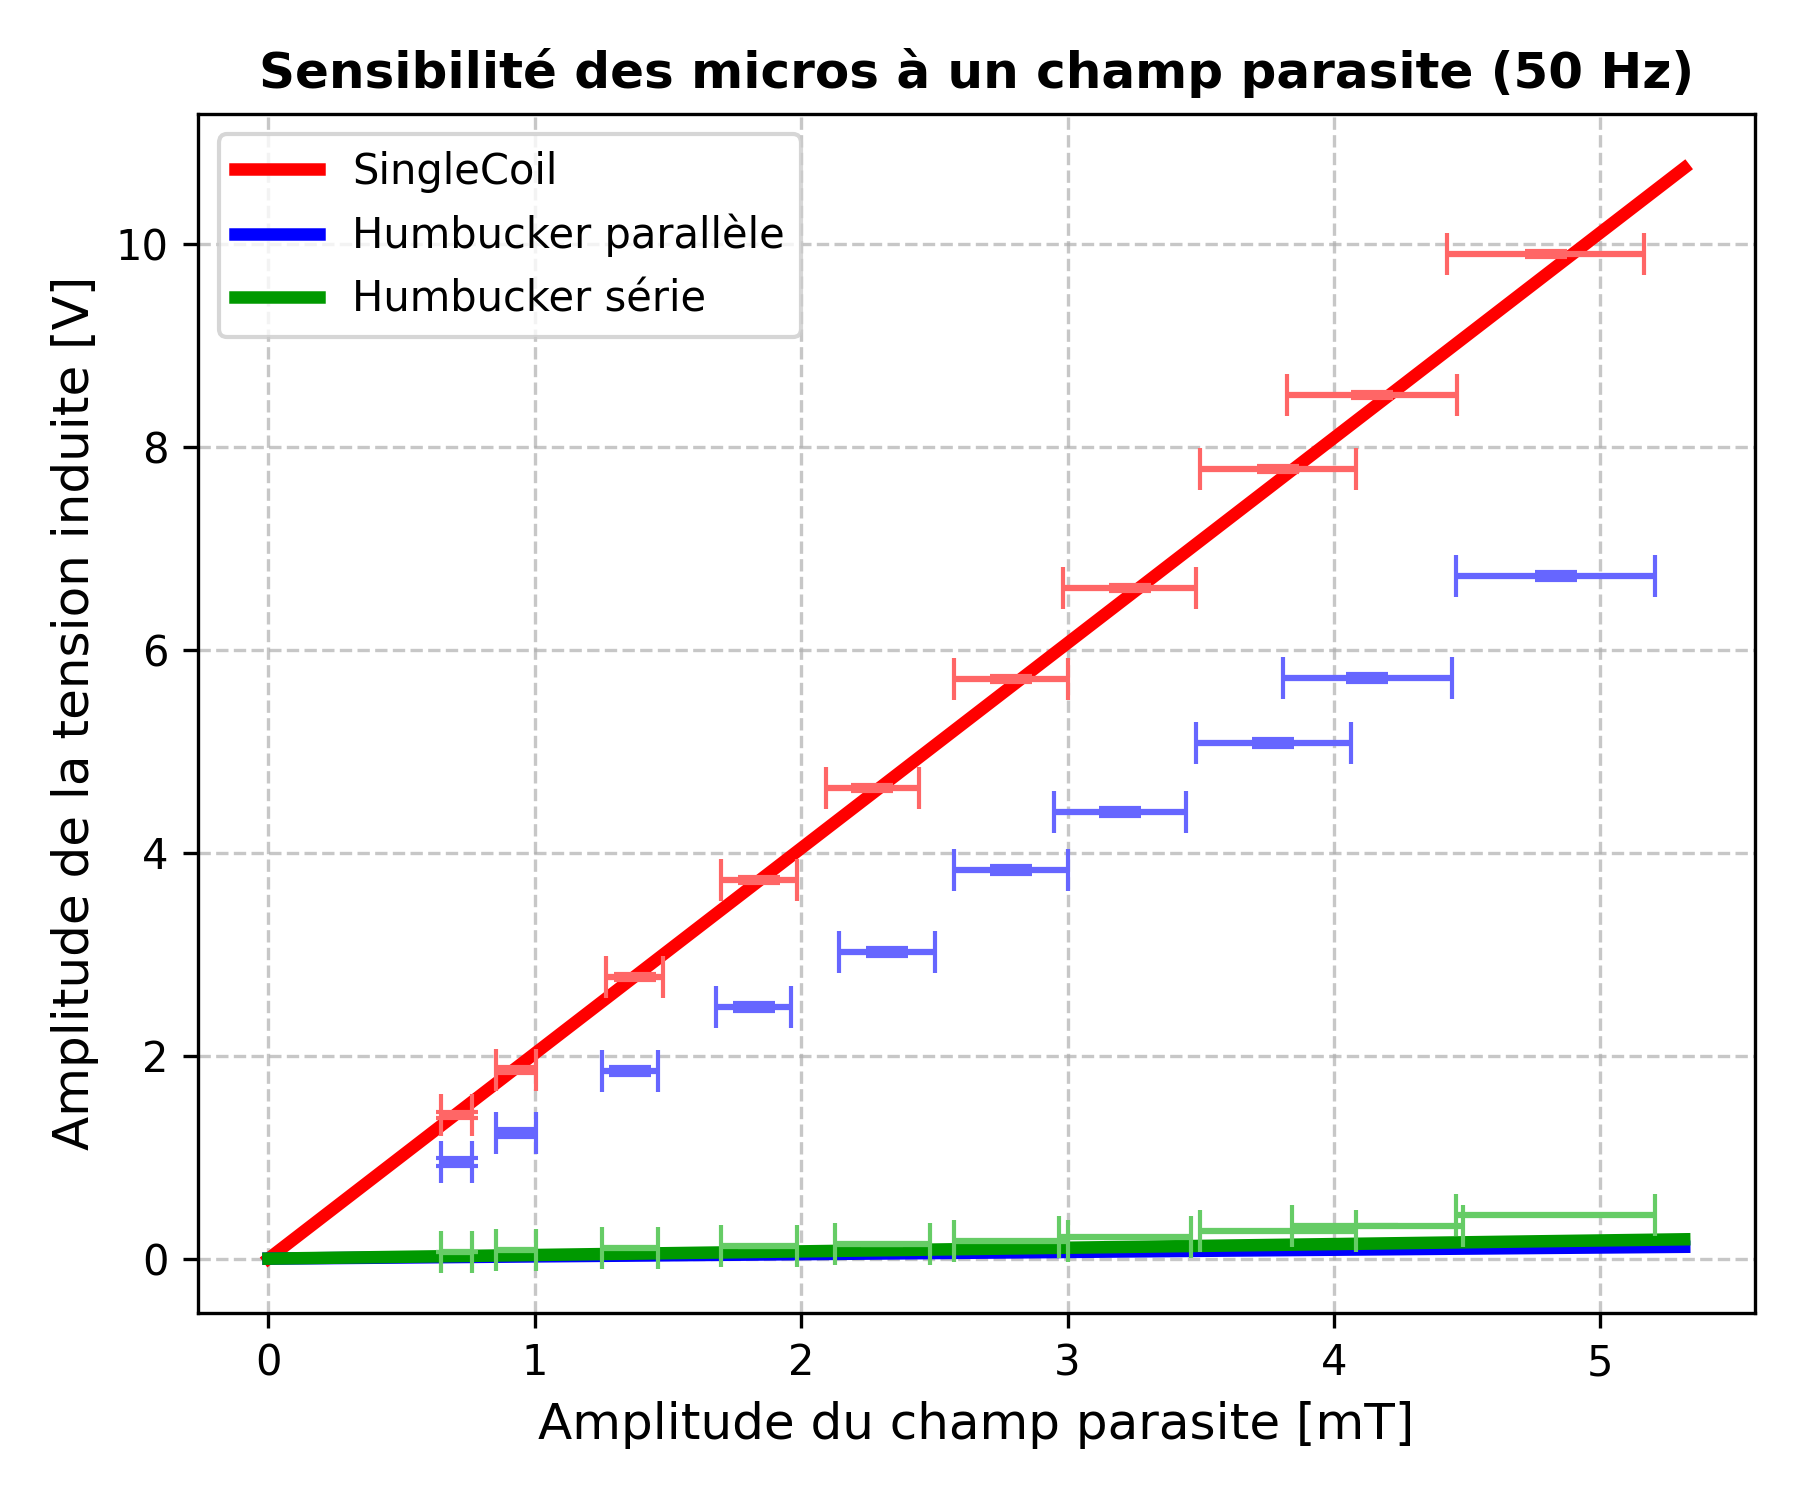
\includegraphics[width=0.8\textwidth]{../../../Python/Exports/03-Reponse_magnetique/Droite_de_sensibilite.png}
    \caption{Sensibilité des micros aux champ magnétique extérieur}
\end{figure}

\subsection{Conclusion}
L'analyse de la rejection des parasites électromagnétiques démontre l'avantage fonctionnel du micro Humbucker, particulièrement dans les contextes exigeants de fortes amplifications. Sur le plan acoustique, cette technologie permet une atténuation marquée du bourdonnement à 50 Hz, un parasite omniprésent dans les environnements de scène ou de studio. Contrairement au SingleCoil, dont la sensibilité élevée aux champs magnétiques ambiants dégrade la qualité du signal, le Humbucker assure une clarté sonore supérieure, même en présence d'interférences électromagnétiques intenses. 

Pour le guitariste, cette caractéristique se traduit par un environnement sonore plus propre, essentiel pour l'exploitation de niveaux de gain élevés sans altération par les parasites. Ainsi, le Humbucker ne se limite pas à une simple amélioration technique : il offre une liberté artistique accrue, en permettant une amplification robuste et un contrôle précis du timbre, même dans des conditions électromagnétiques défavorables. 

Cette étude confirme que le choix entre SingleCoil et Humbucker ne relève pas seulement d'une préférence sonore, mais aussi d'un compromis technique entre richesse harmonique et immunité aux perturbations, un enjeu central pour les musiciens et les luthiers.

\newpage
% --- SECTION IV ---
\section{Conclusion}
Cette étude comparative apporte une réponse quantitative et qualitative à la problématique de l'influence du type de bobinage sur les performances des micros de guitare électrique. L'objectif était d'évaluer dans quelle mesure l'ajout d'une seconde bobine dans le Humbucker permet de concilier l'élimination des parasites électromagnétiques et la préservation de la richesse spectrale du signal induit.

Les résultats démontrent que le micro se comporte comme un filtre passe-bas du second ordre, dont la réponse fréquentielle dépend de ses paramètres intrinsèques. L'identification par l'algorithme de moindre-carre révèle que le SingleCoil présente un pic de résonance marqué, favorisant les hautes fréquences et conférant au son sa brillance caractéristique. Le Humbucker en configuration parallèle, lui, offre une réponse plus linéaire, mais dépourvue du renforcement harmonique dans le spectre audible, expliquant son timbre plus << sombre >>. Puis, le Humbucker en configuration série représente un compromis entre les deux, avec une résonance atténuée mais une meilleure préservation des médiums.

L'analyse de l'induction et du filtrage spatial met en lumière l'influence de la géométrie double du Humbucker. L'espacement $\Delta$ entre les bobines engendre un filtrage en peigne, atténuant sélectivement certaines harmoniques de la corde vibrante. Contrairement au SingleCoil, qui capture fidèlement la vibration mécanique, le Humbucker modifie activement le contenu spectral du signal. Ce phénomène confirme que la perte de brillance observée n'est pas uniquement d'origine électrique, mais résulte d'une interférence destructive inhérente à sa conception spatiale.

L'évaluation du taux de rejection de mode commun (CMRR) valide l'efficacité du Humbucker dans la réduction des parasites. Bien que les mesures expérimentales révèlent un CMRR de 3,5 dB (contre 393 dB en théorie), l'atténuation du bourdonnement à 50 Hz reste significative pour le Humbucker série.

Pour le guitariste, le choix entre SingleCoil et Humbucker représente un compromis fondamental. Le SingleCoil offre une richesse harmonique et une brillance adaptées aux styles exigeant une grande expressivité (ex: blues, funk). Tandis que le Humbucker garantit une stabilité sonore et une immunité aux parasites, essentielles pour les environnements saturés (ex : metal, jazz avec forte amplification).

\newpage
\section{Notations et valeurs numérique}
\subsection{Caractéristiques électriques et mécaniques}
\begin{center}
\small
\begin{tabularx}{\textwidth}{llcX}
\toprule
\textbf{Notation} & \textbf{Valeur} & \textbf{Unité} & \textbf{Description} \\
\midrule
$\mu_{0}$ & $4\pi \cdot 10^{-7}$ & H$\cdot$m$^{-1}$ & Perméabilité magnétique du vide \\
$\mu_{r}$ & 2 & -- & Perméabilité relative de l'Alnico 5 \\
\midrule
$R_{s_S}$ & $5,26 \cdot 10^3$ & $\Omega$ & Résistance interne du micro SingleCoil \\
$L_{S}$ & 2,37 & H & Inductance du micro SingleCoil \\
$C_{S}$ & $0,37 \cdot 10^{-9}$ & F & Capacité interne du micro SingleCoil \\
$R_{p_S}$ & $492,3 \cdot 10^3$ & $\Omega$ & Résistance des pertes par courant de Foucault \\
\midrule
$R_{s_{\text{Hp}}}$ & $4,52 \cdot 10^3$ & $\Omega$ & Résistance interne du micro Humbucker parallèle \\
$L_{\text{Hp}}$ & 1,72 & H & Inductance du micro Humbucker parallèle \\
$C_{\text{Hp}}$ & $0,05 \cdot 10^{-9}$ & F & Capacité interne du micro Humbucker parallèle \\
$R_{p_{\text{Hp}}}$ & $343,0 \cdot 10^3$ & $\Omega$ & Résistance des pertes par courant de Foucault \\
\midrule
$R_{s_{\text{Hs}}}$ & $15,10 \cdot 10^3$ & $\Omega$ & Résistance interne du micro Humbucker série \\
$L_{\text{Hs}}$ & $4,60$ & H & Inductance du micro Humbucker série \\
$C_{\text{Hs}}$ & $0,11 \cdot 10^{-9}$ & F & Capacité interne du micro Humbucker série \\
$R_{p_{\text{Hs}}}$ & $1,05 \cdot 10^6$ & $\Omega$ & Résistance des pertes par courant de Foucault \\
\midrule
$x_{S}$ & 0,105 & m & Position du micro SingleCoil \\
$x_{\text{Hp1}}, x_{\text{Hp2}}$ & 0,147 - 0,165 & m & Position des bobinages du Humbucker parallèle \\
$x_{\text{Hs1}}, x_{\text{Hs2}}$ & 0,202 - 0,220 & m & Position des bobinages du Humbucker série \\
$\Delta$ & 0,018 & m & Entraxe entre les deux bobines du Humbucker \\
\midrule
$z_{0}$ & 0,004 & m & Distance corde micro au repos \\
$L$ & 0,85 & m & Longueur de la corde vibrante \\
$x_{0}$ & 0,20 & m & Position de l'origine de la perturbation \\
$A_{0}$ & 0,005 (ODG) & m & Amplitude initiale de la perturbation \\
$F$ & 80 & Hz & Fréquence fondamentale de vibration de la corde \\
\bottomrule
\end{tabularx}
\end{center}

\subsection{Caractéristiques magnétiques}
\begin{center}
\small
\begin{tabularx}{\textwidth}{llcX}
\toprule
\textbf{Notation} & \textbf{Valeur} & \textbf{Unité} & \textbf{Description} \\
\midrule
$\chi$ & 100 (ODG) & -- & Susceptibilité magnétique de la corde \\
$V$ & $1 \cdot 10^{-8}$ (ODG) & m$^{3}$ & Volume de la portion de la corde active \\
\midrule
$F_{B}$ & 50 & Hz & Fréquence du champ magnétique parasite \\
$\alpha$ & 1 (ODG) & m$^{-1}$ & Gradient du champ magnétique parasite \\
\midrule
$k_{s}$ & 2,02 & $V.mT^{-1}$ & Sensibilité théorique du SingleCoil \\
$k_{\text{Hp}}$ & 0,02 & $V.mT^{-1}$ & Sensibilité théorique du Humbucker parallèle \\
$k_{\text{Hs}}$ & 0,04 & $V.mT^{-1}$ & Sensibilité théorique du Humbucker série \\
$k_{\text{Sexp}}$ & 2,05 & $V.mT^{-1}$ & Sensibilité expérimentale du SingleCoil \\
$k_{\text{Hpexp}}$ & 1,37 & $V.mT^{-1}$ & Sensibilité expérimentale du Humbucker parallèle \\
$k_{\text{Hsexp}}$ & 0,08 & $V.mT^{-1}$ & Sensibilité expérimentale du Humbucker série \\
\midrule
$\text{CMRR}_{Hp}$ & 39,3 & dB & CMRR théorique du Humbucker parallèle \\
$\text{CMRR}_{Hs}$ & 35,0 & dB & CMRR théorique du Humbucker série \\
$\text{CMRR}_{\text{Hpexp}}$ & 3,5 & dB & CMRR expérimentale du Humbucker parallèle \\
$\text{CMRR}_{\text{Hsexp}}$ & 28,7 & dB & CMRR expérimentale du Humbucker série \\
\bottomrule
\end{tabularx}
\end{center}

\newpage
% --- REFERENCES ---
\begin{thebibliography}{9}

\bibitem{wiseguy} 
WiseGuy Research Consultants, \textit{"Global Electric Guitar Pickup Market Research Report 2024,"} Pune, India, 2024.

\bibitem{hill} 
Matthew W. Hill, \textit{"The hidden history of the electric guitar"}, in \textit{Quand la guitare [s']électrise!}, Benoît Navarret et al. (dir.), Sorbonne Université Presses, pp. 33-61, 2022.

\bibitem{horton} 
N. G. Horton \& T. R. Moore: \textit{Modeling the magnetic pickup of an electric guitar} : American Journal of Physics, vol. 77, no. 2, pp. 144-150, 2009, doi: 10.1119/1.2990663.

\bibitem{duncan} 
S. W. Duncan, \textit{"Interview With Seth Lover"}, Seymour Duncan. [En ligne]. Disponible sur : \url{www.seymourduncan.com/blog/latest-updates/seymour-w-duncans-interview-with-seth-lover}

\bibitem{carson} 
Dan Carson, \textit{"Investigation of the Electromagnetic Properties of Electric Guitar Pickups"}, University of Illinois at Urbana-Champaign, Physics Senior Thesis, 2009.

\bibitem{andrea} 
B. d'Andréa-Novel, B. Fabre, et P. Jouvelot, \textit{Acoustique Informatique MusiquE : Outils scientifiques pour la musique}. Paris, France : Presses des Mines, 2010, ch. 4.

\end{thebibliography}

\end{document}